\documentclass[output=paper
,newtxmath
,modfonts
,nonflat]{../langsci/langscibook} 
%\bibliography{localbibliography} 
% \usepackage{pifont}
\usepackage{savesym}

\savesymbol{downingtriple}
\savesymbol{downingdouble}
\savesymbol{downingquad}
\savesymbol{downingquint}
\savesymbol{suph}
\savesymbol{supj}
\savesymbol{supw}
\savesymbol{sups}
\savesymbol{ts}
\savesymbol{tS}
\savesymbol{devi}
\savesymbol{devu}
\savesymbol{devy}
\savesymbol{deva}
\savesymbol{N}
\savesymbol{Z}
\savesymbol{circled}
\savesymbol{sem}
\savesymbol{row}
\savesymbol{tipa}
\savesymbol{tableauxcounter}
\savesymbol{tabhead}
\savesymbol{inp}
\savesymbol{inpno}
\savesymbol{g}
\savesymbol{hanl}
\savesymbol{hanr}
\savesymbol{kuku}
\savesymbol{ip}
\savesymbol{lipm}
\savesymbol{ripm}
\savesymbol{lipn}
\savesymbol{ripn} 
% \usepackage{amsmath} 
% \usepackage{multicol}
\usepackage{qtree} 
\usepackage{tikz-qtree,tikz-qtree-compat}
% \usepackage{tikz}
\usepackage{upgreek}


%%%%%%%%%%%%%%%%%%%%%%%%%%%%%%%%%%%%%%%%%%%%%%%%%%%%
%%%                                              %%%
%%%           Examples                           %%%
%%%                                              %%%
%%%%%%%%%%%%%%%%%%%%%%%%%%%%%%%%%%%%%%%%%%%%%%%%%%%%
% remove the percentage signs in the following lines
% if your book makes use of linguistic examples
\usepackage{tipa}  
\usepackage{pstricks,pst-xkey,pst-asr}

%for sande et al
\usepackage{pst-jtree}
\usepackage{pst-node}
%\usepackage{savesym}


% \usepackage{subcaption}
\usepackage{multirow}  
\usepackage{./langsci/styles/langsci-optional} 
\usepackage{./langsci/styles/langsci-lgr} 
\usepackage{./langsci/styles/langsci-glyphs} 
\usepackage[normalem]{ulem}
%% if you want the source line of examples to be in italics, uncomment the following line
% \def\exfont{\it}
\usetikzlibrary{arrows.meta,topaths,trees}
\usepackage[linguistics]{forest}
\forestset{
	fairly nice empty nodes/.style={
		delay={where content={}{shape=coordinate,for parent={
					for children={anchor=north}}}{}}
}}
\usepackage{soul}
\usepackage{arydshln}
% \usepackage{subfloat}
\usepackage{langsci/styles/langsci-gb4e} 
   
% \usepackage{linguex}
\usepackage{vowel}

\usepackage{pifont}% http://ctan.org/pkg/pifont
\newcommand{\cmark}{\ding{51}}%
\newcommand{\xmark}{\ding{55}}%
 
 
 %Lamont
 \makeatletter
\g@addto@macro\@floatboxreset\centering
\makeatother

\usepackage{newfloat} 
\DeclareFloatingEnvironment[fileext=tbx,name=Tableau]{tableau}
% %% hyphenation points for line breaks
%% Normally, automatic hyphenation in LaTeX is very good
%% If a word is mis-hyphenated, add it to this file
%%
%% add information to TeX file before \begin{document} with:
%% %% hyphenation points for line breaks
%% Normally, automatic hyphenation in LaTeX is very good
%% If a word is mis-hyphenated, add it to this file
%%
%% add information to TeX file before \begin{document} with:
%% %% hyphenation points for line breaks
%% Normally, automatic hyphenation in LaTeX is very good
%% If a word is mis-hyphenated, add it to this file
%%
%% add information to TeX file before \begin{document} with:
%% \include{localhyphenation}
\hyphenation{
affri-ca-te
affri-ca-tes
com-ple-ments
par-a-digm
Sha-ron
Kings-ton
phe-nom-e-non
Daul-ton
Abu-ba-ka-ri
Ngo-nya-ni
Clem-ents 
King-ston
Tru-cken-brodt
Tab-leau
cophono-logies
mark-edness
Ti-gri-nya
a-mong
Car-stens
Lu-bu-ku-su
}
\hyphenation{
affri-ca-te
affri-ca-tes
com-ple-ments
par-a-digm
Sha-ron
Kings-ton
phe-nom-e-non
Daul-ton
Abu-ba-ka-ri
Ngo-nya-ni
Clem-ents 
King-ston
Tru-cken-brodt
Tab-leau
cophono-logies
mark-edness
Ti-gri-nya
a-mong
Car-stens
Lu-bu-ku-su
}
\hyphenation{
affri-ca-te
affri-ca-tes
com-ple-ments
par-a-digm
Sha-ron
Kings-ton
phe-nom-e-non
Daul-ton
Abu-ba-ka-ri
Ngo-nya-ni
Clem-ents 
King-ston
Tru-cken-brodt
Tab-leau
cophono-logies
mark-edness
Ti-gri-nya
a-mong
Car-stens
Lu-bu-ku-su
}
% %add all your local new commands to this file
\newcommand{\downingquad}[4]{\parbox{2.5cm}{#1}\parbox{3.5cm}{#2}\parbox{2.5cm}{#3}\parbox{3.5cm}{#4}}
\newcommand{\downingtriple}[3]{\parbox{4.5cm}{#1}\parbox{3cm}{#2}\parbox{3cm}{#3}}
\newcommand{\downingdouble}[2]{\parbox{4.5cm}{#1}\parbox{6cm}{#2}}
\newcommand{\downingquint}[5]{\parbox{1.75cm}{#1}\parbox{2.25cm}{#2}\parbox{2cm}{#3}\parbox{3cm}{#4}\parbox{2cm}{#5}}
\newcolumntype{Y}{>{\centering\arraybackslash}X}
\newcolumntype{T}{>{\centering\arraybackslash}m{2cm}}

%commands for Kusmer paper below
\newcommand{\ip}{$\upiota$}
\newcommand{\lipm}{(\_{\ip-Max}}
\newcommand{\ripm}{)\_{\ip-Max}}
\newcommand{\lipn}{(\_{\ip}}
\newcommand{\ripn}{)\_{\ip}}
\renewcommand{\_}[1]{\textsubscript{#1}}


%commands for Pillion paper below
\newcommand{\suph}{\textipa{\super h}}
\newcommand{\supj}{\textipa{\super j}}
\newcommand{\supw}{\textipa{\super w}}
\newcommand{\ts}{\textipa{\t{ts}}}
\newcommand{\tS}{\textipa{\t{tS}}}
\newcommand{\devi}{\textipa{\r*i}}
\newcommand{\devu}{\textipa{\r*u}}
\newcommand{\devy}{\textipa{\r*y}}
\newcommand{\deva}{\textipa{\r*a}}
\renewcommand{\N}{\textipa{N}}
\newcommand{\Z}{\textipa{Z}}
% 

%commands for Diercks paper below
\newcommand{\circled}[1]{\begin{tikzpicture}[baseline=(word.base)]
\node[draw, rounded corners, text height=8pt, text depth=2pt, inner sep=2pt, outer sep=0pt, use as bounding box] (word) {#1};
\end{tikzpicture}
}

%commands for Pesetsky paper below
% \newcommand{\sem}[2][]{\mbox{$[\![ $\textbf{#2}$ ]\!]^{#1}$}}
\newcommand{\sem}[2][]{\mbox{$[[ $\textbf{#2}$ ]]^{#1}$}}

% \newcommand{\ripn}{{\color{red}ripn}}%this is used but never defined. Please update the definition



%commands for Lamont paper below
\newcommand{\row}[4]{
	#1. & 
    /{#2}/ & 
    [{#3}] & 
    `#4' \\ 
}
%\newcounter{tableauxcounter}
\newcommand{\tabhead}[2]{
%     \captionsetup{labelformat=empty}
%     \stepcounter{tableauxcounter}
%     \addtocounter{table}{-1}
% 	\centering
% 	\caption{Tableau \thetableauxcounter: #1}
	\caption{#1}
	\label{#2}
}
\newcommand{\candref}[2]{{(\ref{#1}#2)}}
\newcommand{\tableauref}[1]{{Tableau~\ref{#1}}}
% tableaux
\newcommand{\inp}[1]{\multicolumn{2}{|l||}{{#1}}}
\newcommand{\inpno}[1]{\multicolumn{2}{|l||}{#1}}
\newcommand{\g}{\cellcolor{lightgray}}
\newcommand{\hanl}{\HandLeft}
\newcommand{\hanr}{\HandRight}
\newcommand{\kuku}{Kuk\'{u}}

% \newcommand{\nocaption}[1]{{\color{red} Please provide a caption}}

% \providecommand{\biberror}[1]{{\color{red}#1}}

\definecolor{RED}{cmyk}{0.05,1,0.8,0}


\newfontfamily\amharicfont[Script = Ethiopic, Scale = 1.0]{AbyssinicaSIL}
\newcommand{\amh}[1]{{\amharicfont #1}}

% 
% %Gjersoe
\usepackage{textgreek}
% 
\newcommand{\viol}{\fontfamily{MinionPro-OsF}\selectfont\rotatebox{60}{$\star$}}
\newcommand{\myscalex}{0.45}
\newcommand{\myscaley}{0.65}
%\newcommand{\red}[1]{\textcolor{red}{#1}}
%\newcommand{\blue}[1]{\textcolor{blue}{#1}}
\newcommand{\epen}[1]{\colorbox{jgray}{#1}}
\newcommand{\hand}{{\normalsize \ding{43}}}
\definecolor{jgray}{gray}{0.8} 
\usetikzlibrary{positioning}
\usetikzlibrary{matrix}
\newcommand{\mora}{\textmu\xspace}
\newcommand{\si}{\textsigma\xspace}
\newcommand{\ft}{\textPhi\xspace}
\newcommand{\tone}{\texttau\xspace}
\newcommand{\word}{\textomega\xspace}
% \newcommand{\ts}{\texttslig}
\newcommand{\fns}{\footnotesize}
\newcommand{\ns}{\normalsize}
\newcommand{\vs}{\vspace{1em}}
\newcommand{\bs}{\textbackslash}   % backslash
\newcommand{\cmd}[1]{{\bf \color{red}#1}}   % highlights command
\newcommand{\scell}[2][l]{\begin{tabular}[#1]{@{}c@{}}#2\end{tabular}}
% \interfootnotelinepenalty=10000

% --- Snider Representations --- %

\newcommand{\RepLevelHh}{
\begin{minipage}{0.10\textwidth}
\begin{tikzpicture}[xscale=\myscalex,yscale=\myscaley]
%\node (syl) at (0,0) {Hi};
\node (Rt) at (0,1) {o};
\node (H) at (-0.5,2) {H};
\node (R) at (0.5,3) {h};
%\draw [thick] (syl.north) -- (Rt.south) ;
\draw [thick] (Rt.north) -- (H.south) ;
\draw [thick] (Rt.north) -- (R.south) ;
\end{tikzpicture}
\end{minipage}
}

\newcommand{\RepLevelLh}{
\begin{minipage}{0.10\textwidth}
\begin{tikzpicture}[xscale=\myscalex,yscale=\myscaley]
%\node (syl) at (0,0) {Mid2};
\node (Rt) at (0,1) {o};
\node (H) at (-0.5,2) {L};
\node (R) at (0.5,3) {h};
%\draw [thick] (syl.north) -- (Rt.south) ;
\draw [thick] (Rt.north) -- (H.south) ;
\draw [thick] (Rt.north) -- (R.south) ;
\end{tikzpicture}
\end{minipage}
}

\newcommand{\RepLevelHl}{
\begin{minipage}{0.10\textwidth}
\begin{tikzpicture}[xscale=\myscalex,yscale=\myscaley]
%\node (syl) at (0,0) {Mid1};
\node (Rt) at (0,1) {o};
\node (H) at (-0.5,2) {H};
\node (R) at (0.5,3) {l};
%\draw [thick] (syl.north) -- (Rt.south) ;
\draw [thick] (Rt.north) -- (H.south) ;
\draw [thick] (Rt.north) -- (R.south) ;
\end{tikzpicture}
\end{minipage}
}

\newcommand{\RepLevelLl}{
\begin{minipage}{0.10\textwidth}
\begin{tikzpicture}[xscale=\myscalex,yscale=\myscaley]
%\node (syl) at (0,0) {Lo};
\node (Rt) at (0,1) {o};
\node (H) at (-0.5,2) {L};
\node (R) at (0.5,3) {l};
%\draw [thick] (syl.north) -- (Rt.south) ;
\draw [thick] (Rt.north) -- (H.south) ;
\draw [thick] (Rt.north) -- (R.south) ;
\end{tikzpicture}
\end{minipage}
}

% --- Representations --- %

\newcommand{\RepLevel}{
\begin{minipage}{0.10\textwidth}
\begin{tikzpicture}[xscale=\myscalex,yscale=\myscaley]
\node (syl) at (0,0) {\textsigma};
\node (Rt) at (0,1) {o};
\node (H) at (-0.5,2) {\texttau};
\node (R) at (0.5,3) {\textrho};
\draw [thick] (syl.north) -- (Rt.south) ;
\draw [thick] (Rt.north) -- (H.south) ;
\draw [thick] (Rt.north) -- (R.south) ;
\end{tikzpicture}
\end{minipage}
}

\newcommand{\RepContour}{
\begin{minipage}{0.10\textwidth}
\begin{tikzpicture}[xscale=\myscalex,yscale=\myscaley]
\node (syl) at (0,0) {\textsigma};
\node (Rt) at (0,1) {o};
\node (H) at (-0.5,2) {\texttau};
\node (R) at (0.5,3) {\textrho};
\node (Rt2) at (1.5,1.0) {o};
%\node (H2) at (1.0,2) {$\tau$};
%\node (R2) at (2.0,2.5) {R};
\draw [thick] (syl.north) -- (Rt.south) ;
\draw [thick] (Rt.north) -- (H.south) ;
\draw [thick] (Rt.north) -- (R.south) ;
\draw [thick] (syl.north) -- (Rt2.south) ;
%\draw [thick] (Rt2.north) -- (H2.south) ;
%\draw [thick] (Rt2.north) -- (R2.south) ;
\end{tikzpicture}
\end{minipage}
}


% --- OT constraints --- %

\newcommand{\IllustrationDown}{
\begin{minipage}{0.09\textwidth}
\begin{tikzpicture}[xscale=0.7,yscale=0.45]
\node (reg) at (0,0.75) {{\small \textalpha}};
\node (arrow) at (0,0) {{\fns $\downarrow$}};
\node (Rt) at (0,-0.75) {{\small \textbeta}};
\end{tikzpicture}
\end{minipage}
}

\newcommand{\IllustrationUp}{
\begin{minipage}{0.09\textwidth}
\begin{tikzpicture}[xscale=0.7,yscale=0.45]
\node (reg) at (0,0.75) {{\small \textalpha}};
\node (arrow) at (0,0) {{\fns $\uparrow$}};
\node (Rt) at (0,-0.75) {{\small \textbeta}};
\end{tikzpicture}
\end{minipage}
}

\newcommand{\MaxAB}{
\begin{minipage}{0.09\textwidth}
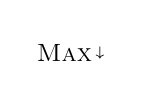
\begin{tikzpicture}[xscale=0.6,yscale=0.4]
\node (max) at (0,0) {{\small \textsc{Max}}};
\node (reg) at (0.75,0.5) {{\fns \textalpha}};
\node (arrow) at (0.75,0) {{\tiny $\downarrow$}};
\node (Rt) at (0.75,-0.5) {{\fns \textbeta}};
\end{tikzpicture}
\end{minipage}
}

\newcommand{\DepAB}{
\begin{minipage}{0.09\textwidth}
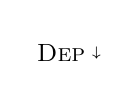
\begin{tikzpicture}[xscale=0.6,yscale=0.4]
\node (max) at (0,0) {{\small \textsc{Dep}}};
\node (reg) at (0.75,0.5) {{\fns \textalpha}};
\node (arrow) at (0.75,0) {{\tiny $\downarrow$}};
\node (Rt) at (0.75,-0.5) {{\fns \textbeta}};
\end{tikzpicture}
\end{minipage}
}

\newcommand{\DepHReg}{
\begin{minipage}{0.055\textwidth}
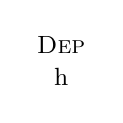
\begin{tikzpicture}[xscale=0.6,yscale=0.4]
\node (dep) at (0,0) {{\small \textsc{Dep}}};
\node (reg) at (0,-1.0) {{\small h}};
\end{tikzpicture}
\end{minipage}
}

\newcommand{\DepLReg}{
\begin{minipage}{0.055\textwidth}
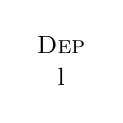
\begin{tikzpicture}[xscale=0.6,yscale=0.4]
\node (dep) at (0,0) {{\small \textsc{Dep}}};
\node (reg) at (0,-1.0) {{\small l}};
\end{tikzpicture}
\end{minipage}
}

\newcommand{\DepReg}{
\begin{minipage}{0.055\textwidth}
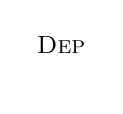
\begin{tikzpicture}[xscale=0.6,yscale=0.4]
\node (dep) at (0,0) {{\small \textsc{Dep}}};
\node (reg) at (0,-1.0) {{\small \textrho}};
\end{tikzpicture}
\end{minipage}
}

\newcommand{\DepTRt}{
\begin{minipage}{0.1\textwidth}
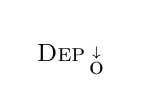
\begin{tikzpicture}[xscale=0.6,yscale=0.4]
\node (dep) at (0,0) {{\small \textsc{Dep}}};
\node (t) at (0.75,0.5) {{\fns \texttau}};
\node (arrow) at (0.75,0) {{\tiny $\downarrow$}};
\node (Rt) at (0.75,-0.5) {{\fns o}};
\end{tikzpicture}
\end{minipage}
}

\newcommand{\MaxRegRt}{
\begin{minipage}{0.1\textwidth}
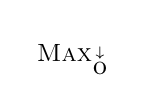
\begin{tikzpicture}[xscale=0.6,yscale=0.4]
\node (max) at (0,0) {{\small \textsc{Max}}};
\node (arrow) at (0.75,0) {{\tiny $\downarrow$}};
\node (Rt) at (0.75,-0.5) {{\fns o}};
\node (reg) at (0.75,0.5) {{\fns \textrho}};
\end{tikzpicture}
\end{minipage}
}

\newcommand{\RegToneByRt}{
\begin{minipage}{0.06\textwidth}
\begin{tikzpicture}[xscale=0.6,yscale=0.5]
\node[rotate=20] (arrow1) at (-0.15,0) {{\fns $\uparrow$}};
\node[rotate=340] (arrow2) at (0.15,0) {{\fns $\uparrow$}};
\node (Rt) at (0,-0.55) {{\small o}};
\node (reg) at (0.4,0.55) {{\small \textrho}};
\node (tone) at (-0.4,0.55) {{\small \texttau}};
\end{tikzpicture}
\end{minipage}
}

\newcommand{\RegToneBySyl}{
\begin{minipage}{0.06\textwidth}
\begin{tikzpicture}[xscale=0.6,yscale=0.5]
\node[rotate=20] (arrow1) at (-0.15,0) {{\fns $\uparrow$}};
\node[rotate=340] (arrow2) at (0.15,0) {{\fns $\uparrow$}};
\node (Rt) at (0,-0.55) {{\small \textsigma}};
\node (reg) at (0.4,0.55) {{\small \textrho}};
\node (tone) at (-0.4,0.55) {{\small \texttau}};
\end{tikzpicture}
\end{minipage}
}

\newcommand{\DepTone}{
\begin{minipage}{0.055\textwidth}
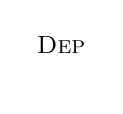
\begin{tikzpicture}[xscale=0.6,yscale=0.4]
\node (dep) at (0,0) {{\small \textsc{Dep}}};
\node (tone) at (0,-1.0) {{\small \texttau}};
\end{tikzpicture}
\end{minipage}
}

\newcommand{\DepTonalRt}{
\begin{minipage}{0.055\textwidth}
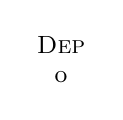
\begin{tikzpicture}[xscale=0.6,yscale=0.4]
\node (dep) at (0,0) {{\small \textsc{Dep}}};
\node (tone) at (0,-1.0) {{\small o}};
\end{tikzpicture}
\end{minipage}
}

\newcommand{\DepL}{
\begin{minipage}{0.055\textwidth}
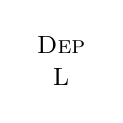
\begin{tikzpicture}[xscale=0.6,yscale=0.4]
\node (dep) at (0,0) {{\small \textsc{Dep}}};
\node (tone) at (0,-1.0) {{\small L}};
\end{tikzpicture}
\end{minipage}
}

\newcommand{\DepH}{
\begin{minipage}{0.055\textwidth}
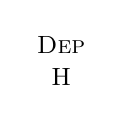
\begin{tikzpicture}[xscale=0.6,yscale=0.4]
\node (dep) at (0,0) {{\small \textsc{Dep}}};
\node (tone) at (0,-1.0) {{\small H}};
\end{tikzpicture}
\end{minipage}
}

\newcommand{\NoMultDiff}{{\small *loh}}
\newcommand{\Alt}{{\small \textsc{Alt}}}
\newcommand{\NoSkip}{{\small \scell{\textsc{No}\\\textsc{Skip}}}}


\newcommand{\RegDomRt}{
\begin{minipage}{0.030\textwidth}
\begin{tikzpicture}[xscale=0.6,yscale=0.5]
\node (arrow) at (0,0) {{\fns $\downarrow$}};
\node (Rt) at (0,-0.55) {{\small o}};
\node (reg) at (0,0.55) {{\small \textrho}};
\end{tikzpicture}
\end{minipage}
}

\newcommand{\DepRegRt}{
\begin{minipage}{0.1\textwidth}
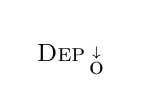
\begin{tikzpicture}[xscale=0.6,yscale=0.4]
\node (dep) at (0,0) {{\small \textsc{Dep}}};
\node (arrow) at (0.75,0) {{\tiny $\downarrow$}};
\node (Rt) at (0.75,-0.5) {{\fns o}};
\node (reg) at (0.75,0.5) {{\fns \textrho}};
\end{tikzpicture}
\end{minipage}
}

% unused

\newcommand{\ToneByRt}{
\begin{minipage}{0.05\textwidth}
\begin{tikzpicture}[xscale=0.6,yscale=0.5]
\node (arrow) at (0,0) {{\fns $\uparrow$}};
\node (Rt) at (0,-0.55) {{\small o}};
\node (tone) at (0,0.55) {{\small \texttau}};
\end{tikzpicture}
\end{minipage}
}

\newcommand{\RegByRt}{
\begin{minipage}{0.05\textwidth}
\begin{tikzpicture}[xscale=0.6,yscale=0.5]
\node (arrow) at (0,0) {{\fns $\uparrow$}};
\node (Rt) at (0,-0.55) {{\small o}};
\node (reg) at (0,0.55) {{\small \textrho}};
\end{tikzpicture}
\end{minipage}
}

\newcommand{\ToneDomRt}{
\begin{minipage}{0.05\textwidth}
\begin{tikzpicture}[xscale=0.6,yscale=0.5]
\node (arrow) at (0,0) {{\fns $\downarrow$}};
\node (Rt) at (0,-0.55) {{\small o}};
\node (tone) at (0,0.55) {{\small \texttau}};
\end{tikzpicture}
\end{minipage}
}

% --- OT tableaus --- %

% Sec. 3.2, first tabl.

\newcommand{\OTHLInput}{
\begin{minipage}{0.17\textwidth}
\begin{tikzpicture}[xscale=\myscalex,yscale=\myscaley]
\node (tone) at (2,0) {(= H)};
\node (syl) at (0,0) {\textsigma};
\node (Rt) at (0,1) {o};
\node (H) at (-0.5,2) {H};
\node (R) at (0.5,3) {h};
\node (Rt2) at (1.5,1.0) {o};
%\node (H2) at (1.0,2) {\epen{L}};
\node (R2) at (2.0,3) {\blue{l}};
\draw [thick] (syl.north) -- (Rt.south) ;
\draw [thick] (Rt.north) -- (H.south) ;
\draw [thick] (Rt.north) -- (R.south) ;
\draw [thick] (syl.north) -- (Rt2.south) ;
%\draw [dashed] (Rt2.north) -- (H2.south) ;
%\draw [dashed] (Rt2.north) -- (R2.south) ;
\end{tikzpicture}
\end{minipage}
}

\newcommand{\OTHLWinner}{
\begin{minipage}{0.17\textwidth}
\begin{tikzpicture}[xscale=\myscalex,yscale=\myscaley]
\node (tone) at (2,0) {(= HL)};
\node (syl) at (0,0) {\textsigma};
\node (Rt) at (0,1) {o};
\node (H) at (-0.5,2) {H};
\node (R) at (0.5,3) {h};
\node (Rt2) at (1.5,1.0) {o};
\node (H2) at (1.0,2) {\epen{L}};
\node (R2) at (2.0,3) {\blue{l}};
\draw [thick] (syl.north) -- (Rt.south) ;
\draw [thick] (Rt.north) -- (H.south) ;
\draw [thick] (Rt.north) -- (R.south) ;
\draw [thick] (syl.north) -- (Rt2.south) ;
\draw [dashed] (Rt2.north) -- (H2.south) ;
\draw [dashed] (Rt2.north) -- (R2.south) ;
\end{tikzpicture}
\end{minipage}
}

\newcommand{\OTHLSpreadingHOnly}{
\begin{minipage}{0.17\textwidth}
\begin{tikzpicture}[xscale=\myscalex,yscale=\myscaley]
\node (tone) at (2,0) {(= HM)};
\node (syl) at (0,0) {\textsigma};
\node (Rt) at (0,1) {o};
\node (H) at (-0.5,2) {H};
\node (R) at (0.5,3) {h};
\node (Rt2) at (1.5,1.0) {o};
%\node (H2) at (1.0,2) {\epen{L}};
\node (R2) at (2.0,3) {\blue{l}};
\draw [thick] (syl.north) -- (Rt.south) ;
\draw [thick] (Rt.north) -- (H.south) ;
\draw [thick] (Rt.north) -- (R.south) ;
\draw [thick] (syl.north) -- (Rt2.south) ;
\draw [dashed] (Rt2.north) -- (R2.south) ;
\draw [dashed] (Rt2.north) -- (H.south) ;
\end{tikzpicture}
\end{minipage}
}

\newcommand{\OTHLInsertH}{
\begin{minipage}{0.17\textwidth}
\begin{tikzpicture}[xscale=\myscalex,yscale=\myscaley]
\node (tone) at (2,0) {(= HM)};
\node (syl) at (0,0) {\textsigma};
\node (Rt) at (0,1) {o};
\node (H) at (-0.5,2) {H};
\node (R) at (0.5,3) {h};
\node (Rt2) at (1.5,1.0) {o};
\node (H2) at (1.0,2) {\epen{H}};
\node (R2) at (2.0,3) {\blue{l}};
\draw [thick] (syl.north) -- (Rt.south) ;
\draw [thick] (Rt.north) -- (H.south) ;
\draw [thick] (Rt.north) -- (R.south) ;
\draw [thick] (syl.north) -- (Rt2.south) ;
\draw [dashed] (Rt2.north) -- (H2.south) ;
\draw [dashed] (Rt2.north) -- (R2.south) ;
\end{tikzpicture}
\end{minipage}
}

\newcommand{\OTHLOverwriting}{
\begin{minipage}{0.17\textwidth}
\begin{tikzpicture}[xscale=\myscalex,yscale=\myscaley]
\node (syl) at (0,0) {\textsigma};
\node (Rt) at (0,1) {o};
\node (H) at (-0.5,2) {H};
\node (R) at (0.5,3) {h};
\node (Rt2) at (1.5,1.0) {o};
%\node (H2) at (1.0,2) {\epen{L}};
\node (R2) at (2.0,3) {\blue{l}};
\draw [thick] (syl.north) -- (Rt.south) ;
\draw [thick] (Rt.north) -- (H.south) ;
\draw [thick] (Rt.north) -- (R.south) ;
\draw [thick] (syl.north) -- (Rt2.south) ;
%\draw [dashed] (Rt2.north) -- (H2.south) ;
\draw [dashed] (Rt.north) -- (R2.south) ;
\node (del) at (0.3,1.9) {\textbf{=}};
\end{tikzpicture}
\end{minipage}
}

\newcommand{\OTHLSpreading}{
\begin{minipage}{0.17\textwidth}
\begin{tikzpicture}[xscale=\myscalex,yscale=\myscaley]
\node (syl) at (0,0) {\textsigma};
\node (Rt) at (0,1) {o};
\node (H) at (-0.5,2) {H};
\node (R) at (0.5,3) {h};
\node (Rt2) at (1.5,1.0) {o};
%\node (H2) at (1.0,2) {\epen{L}};
\node (R2) at (2.0,3) {\blue{l}};
\draw [thick] (syl.north) -- (Rt.south) ;
\draw [thick] (Rt.north) -- (H.south) ;
\draw [thick] (Rt.north) -- (R.south) ;
\draw [thick] (syl.north) -- (Rt2.south) ;
%\draw [dashed] (Rt2.north) -- (H2.south) ;
\draw [dashed] (Rt2.north) -- (H.south) ;
\draw [dashed] (Rt2.north) -- (R.south) ;
\end{tikzpicture}
\end{minipage}
}

% Sec. 4.2, second tabl.: phrase-medial position

\newcommand{\OTHnoLInput}{
\begin{minipage}{0.17\textwidth}
\begin{tikzpicture}[xscale=\myscalex,yscale=\myscaley]
\node (tone) at (2,0) {(= H)};
\node (syl) at (0,0) {\textsigma};
\node (Rt) at (0,1) {o};
\node (H) at (-0.5,2) {H};
\node (R) at (0.5,3) {h};
\node (Rt2) at (1.5,1.0) {o};
%\node (H2) at (1.0,2) {\epen{L}};
%\node (R2) at (2.0,3) {\blue{l}};
\draw [thick] (syl.north) -- (Rt.south) ;
\draw [thick] (Rt.north) -- (H.south) ;
\draw [thick] (Rt.north) -- (R.south) ;
\draw [thick] (syl.north) -- (Rt2.south) ;
\end{tikzpicture}
\end{minipage}
}

\newcommand{\OTHnoLEpenth}{
\begin{minipage}{0.17\textwidth}
\begin{tikzpicture}[xscale=\myscalex,yscale=\myscaley]
\node (tone) at (2,0) {(= HM)};
\node (syl) at (0,0) {\textsigma};
\node (Rt) at (0,1) {o};
\node (H) at (-0.5,2) {H};
\node (R) at (0.5,3) {h};
\node (Rt2) at (1.5,1.0) {o};
\node (H2) at (1.0,2) {\epen{L}};
\node (R2) at (2.0,3) {\epen{h}};
\draw [thick] (syl.north) -- (Rt.south) ;
\draw [thick] (Rt.north) -- (H.south) ;
\draw [thick] (Rt.north) -- (R.south) ;
\draw [thick] (syl.north) -- (Rt2.south) ;
\draw [dashed] (Rt2.north) -- (H2.south) ;
\draw [dashed] (Rt2.north) -- (R2.south) ;
\end{tikzpicture}
\end{minipage}
}

\newcommand{\OTHnoLSpreading}{
\begin{minipage}{0.17\textwidth}
\begin{tikzpicture}[xscale=\myscalex,yscale=\myscaley]
\node (tone) at (2,0) {(= HH)};
\node (syl) at (0,0) {\textsigma};
\node (Rt) at (0,1) {o};
\node (H) at (-0.5,2) {H};
\node (R) at (0.5,3) {h};
\node (Rt2) at (1.5,1.0) {o};
%\node (H2) at (1.0,2) {\epen{L}};
%\node (R2) at (2.0,3) {\blue{l}};
\draw [thick] (syl.north) -- (Rt.south) ;
\draw [thick] (Rt.north) -- (H.south) ;
\draw [thick] (Rt.north) -- (R.south) ;
\draw [thick] (syl.north) -- (Rt2.south) ;
\draw [dashed] (Rt2.north) -- (H.south) ;
\draw [dashed] (Rt2.north) -- (R.south) ;
\end{tikzpicture}
\end{minipage}
}

% Sec. 4.2, third tabl., LM is unaffected by L\%

\newcommand{\OTLMInput}{
\begin{minipage}{0.2\textwidth}
\begin{tikzpicture}[xscale=\myscalex,yscale=\myscaley]
\node (tone) at (2,0) {(= LM)};
\node (syl) at (0,0) {\textsigma};
\node (Rt) at (0,1) {o};
\node (H) at (-0.5,2) {L};
\node (R) at (0.5,3) {l};
\node (Rt2) at (1.5,1.0) {o};
\node (H2) at (1.0,2) {L};
\node (R2) at (2.0,3) {h};
\node (R3) at (3.0,3) {\blue{l}};
\draw [thick] (syl.north) -- (Rt.south) ;
\draw [thick] (Rt.north) -- (H.south) ;
\draw [thick] (Rt.north) -- (R.south) ;
\draw [thick] (syl.north) -- (Rt2.south) ;
\draw [thick] (Rt2.north) -- (H2.south) ;
\draw [thick] (Rt2.north) -- (R2.south) ;
\end{tikzpicture}
\end{minipage}
}

\newcommand{\OTLMReplace}{
\begin{minipage}{0.2\textwidth}
\begin{tikzpicture}[xscale=\myscalex,yscale=\myscaley]
\node (tone) at (2,0) {(= LL)};
\node (syl) at (0,0) {\textsigma};
\node (Rt) at (0,1) {o};
\node (H) at (-0.5,2) {L};
\node (R) at (0.5,3) {l};
\node (Rt2) at (1.5,1.0) {o};
\node (H2) at (1.0,2) {L};
\node (R2) at (2.0,3) {h};
\node (R3) at (3.0,3) {\blue{l}};
\draw [thick] (syl.north) -- (Rt.south) ;
\draw [thick] (Rt.north) -- (H.south) ;
\draw [thick] (Rt.north) -- (R.south) ;
\draw [thick] (syl.north) -- (Rt2.south) ;
\draw [thick] (Rt2.north) -- (H2.south) ;
\draw [thick] (Rt2.north) -- (R2.south) ;
\draw [dashed] (Rt2.north) -- (R3.south) ;
\node (del) at (1.8,2.1) {\textbf{=}};
\end{tikzpicture}
\end{minipage}
}

\newcommand{\OTLMTwoReg}{
\begin{minipage}{0.2\textwidth}
\begin{tikzpicture}[xscale=\myscalex,yscale=\myscaley]
\node (tone) at (2,0) {(= LML)};
\node (syl) at (0,0) {\textsigma};
\node (Rt) at (0,1) {o};
\node (H) at (-0.5,2) {L};
\node (R) at (0.5,3) {l};
\node (Rt2) at (1.5,1.0) {o};
\node (H2) at (1.0,2) {L};
\node (R2) at (2.0,3) {h};
\node (R3) at (3.0,3) {\blue{l}};
\draw [thick] (syl.north) -- (Rt.south) ;
\draw [thick] (Rt.north) -- (H.south) ;
\draw [thick] (Rt.north) -- (R.south) ;
\draw [thick] (syl.north) -- (Rt2.south) ;
\draw [thick] (Rt2.north) -- (H2.south) ;
\draw [thick] (Rt2.north) -- (R2.south) ;
\draw [dashed] (Rt2.north) -- (R3.south) ;
\end{tikzpicture}
\end{minipage}
}

% Sec. 4.2, fourth tabl., L is affected by L\% but M is not

\newcommand{\OTLInput}{
\begin{minipage}{0.17\textwidth}
\begin{tikzpicture}[xscale=\myscalex,yscale=\myscaley]
\node (tone) at (2,0) {(= L)};
\node (syl) at (0,0) {\textsigma};
\node (Rt) at (0,1) {o};
\node (H) at (-0.5,2) {L};
\node (R) at (0.5,3) {l};
\node (R2) at (2,3) {\blue{l}};
\draw [thick] (syl.north) -- (Rt.south) ;
\draw [thick] (Rt.north) -- (H.south) ;
\draw [thick] (Rt.north) -- (R.south) ;
\end{tikzpicture}
\end{minipage}
}

\newcommand{\OTLLowered}{
\begin{minipage}{0.17\textwidth}
\begin{tikzpicture}[xscale=\myscalex,yscale=\myscaley]
\node (tone) at (2,0) {(= LL)};
\node (syl) at (0,0) {\textsigma};
\node (Rt) at (0,1) {o};
\node (H) at (-0.5,2) {L};
\node (R) at (0.5,3) {l};
\node (R2) at (2,3) {\blue{l}};
\draw [thick] (syl.north) -- (Rt.south) ;
\draw [thick] (Rt.north) -- (H.south) ;
\draw [thick] (Rt.north) -- (R.south) ;
\draw [dashed] (Rt.north) -- (R2.south) ;
\end{tikzpicture}
\end{minipage}
}

\newcommand{\OTMInput}{
\begin{minipage}{0.17\textwidth}
\begin{tikzpicture}[xscale=\myscalex,yscale=\myscaley]
\node (tone) at (2,0) {(= M)};
\node (syl) at (0,0) {\textsigma};
\node (Rt) at (0,1) {o};
\node (H) at (-0.5,2) {L};
\node (R) at (0.5,3) {h};
\node (R2) at (2,3) {\blue{l}};
\draw [thick] (syl.north) -- (Rt.south) ;
\draw [thick] (Rt.north) -- (H.south) ;
\draw [thick] (Rt.north) -- (R.south) ;
\end{tikzpicture}
\end{minipage}
}

\newcommand{\OTMLowered}{
\begin{minipage}{0.17\textwidth}
\begin{tikzpicture}[xscale=\myscalex,yscale=\myscaley]
\node (tone) at (2,0) {(= ML)};
\node (syl) at (0,0) {\textsigma};
\node (Rt) at (0,1) {o};
\node (H) at (-0.5,2) {L};
\node (R) at (0.5,3) {h};
\node (R2) at (2,3) {\blue{l}};
\draw [thick] (syl.north) -- (Rt.south) ;
\draw [thick] (Rt.north) -- (H.south) ;
\draw [thick] (Rt.north) -- (R.south) ;
\draw [dashed] (Rt.north) -- (R2.south) ;
\end{tikzpicture}
\end{minipage}
}

% Sec. 4.2, fifth tableau, polar questions with level tones

\newcommand{\OTLPolIn}{
\begin{minipage}{0.20\textwidth}
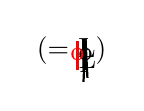
\begin{tikzpicture}[xscale=\myscalex-0.05,yscale=\myscaley-0.05]
\node (tone) at (3.5,0) {(= L)};
\node (syl) at (0,0) {\textsigma};
\node (syl2) at (2,0) {\red{\textsigma}};
\node (Rt) at (0,1) {o};
\node (H) at (-0.5,2) {L};
\node (R) at (0.5,3) {l};
\node (Rt2) at (2,1) {\red{o}};
\draw [thick] (syl.north) -- (Rt.south) ;
\draw [thick,red] (syl2.north) -- (Rt2.south) ;
\draw [thick] (Rt.north) -- (H.south) ;
\draw [thick] (Rt.north) -- (R.south) ;
\end{tikzpicture}
\end{minipage}
}

\newcommand{\OTLPolDef}{
\begin{minipage}{0.20\textwidth}
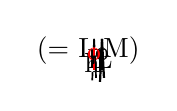
\begin{tikzpicture}[xscale=\myscalex-0.05,yscale=\myscaley-0.05]
\node (tone) at (3.5,0) {(= L.M)};
\node (syl) at (0,0) {\textsigma};
\node (syl2) at (2,0) {\red{\textsigma}};
\node (Rt) at (0,1) {o};
\node (H) at (-0.5,2) {L};
\node (R) at (0.5,3) {l};
\node (H2) at (1.5,2) {\epen{L}};
\node (R2) at (2.5,3) {\epen{h}};
\node (Rt2) at (2,1) {\red{o}};
\draw [thick] (syl.north) -- (Rt.south) ;
\draw [thick,red] (syl2.north) -- (Rt2.south) ;
\draw [thick] (Rt.north) -- (H.south) ;
\draw [thick] (Rt.north) -- (R.south) ;
\draw [semithick,dashed] (Rt2.north) -- (H2.south) ;
\draw [semithick,dashed] (Rt2.north) -- (R2.south) ;
\end{tikzpicture}
\end{minipage}
}

\newcommand{\OTLPolAlt}{
\begin{minipage}{0.20\textwidth}
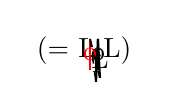
\begin{tikzpicture}[xscale=\myscalex-0.05,yscale=\myscaley-0.05]
\node (tone) at (3.5,0) {(= L.L)};
\node (syl) at (0,0) {\textsigma};
\node (syl2) at (2,0) {\red{\textsigma}};
\node (Rt) at (0,1) {o};
\node (H) at (-0.5,2) {L};
\node (R) at (0.5,3) {l};
\node (Rt2) at (2,1) {\red{o}};
\draw [thick] (syl.north) -- (Rt.south) ;
\draw [thick,red] (syl2.north) -- (Rt2.south) ;
\draw [thick] (Rt.north) -- (H.south) ;
\draw [thick] (Rt.north) -- (R.south) ;
\draw [semithick,dashed] (Rt2.north) -- (H.south) ;
\draw [semithick,dashed] (Rt2.north) -- (R.south) ;
\end{tikzpicture}
\end{minipage}
}

% Sec. 4.2, sixth tableau, polar questions with contour tones

\newcommand{\OTLLPolIn}{
\begin{minipage}{0.23\textwidth}
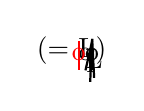
\begin{tikzpicture}[xscale=\myscalex-0.05,yscale=\myscaley-0.05]
\node (tone) at (5.2,0) {(= L)};
\node (syl) at (0,0) {\textsigma};
\node (syl3) at (3.4,0) {\red{\textsigma}};
\node (Rt) at (0,1) {o};
\node (Rt2) at (1.7,1) {o};
\node (Rt3) at (3.4,1) {\red{o}};
\node (H) at (-0.5,2) {L};
\node (R) at (0.5,3) {l};
\draw [thick] (syl.north) -- (Rt.south) ;
\draw [thick] (syl.north) -- (Rt2.south) ;
\draw [thick,red] (syl3.north) -- (Rt3.south) ;
\draw [thick] (Rt.north) -- (H.south) ;
\draw [thick] (Rt.north) -- (R.south) ;
\end{tikzpicture}
\end{minipage}
}

\newcommand{\OTLLPolDef}{
\begin{minipage}{0.23\textwidth}
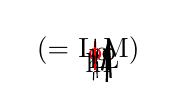
\begin{tikzpicture}[xscale=\myscalex-0.05,yscale=\myscaley-0.05]
\node (tone) at (5.2,0) {(= L.M)};
\node (syl) at (0,0) {\textsigma};
\node (syl3) at (3.4,0) {\red{\textsigma}};
\node (Rt) at (0,1) {o};
\node (Rt2) at (1.7,1) {o};
\node (Rt3) at (3.4,1) {\red{o}};
\node (H) at (-0.5,2) {L};
\node (R) at (0.5,3) {l};
\node (H3) at (2.9,2) {\epen{L}};
\node (R3) at (3.9,3) {\epen{h}};
\draw [thick] (syl.north) -- (Rt.south) ;
\draw [thick] (syl.north) -- (Rt2.south) ;
\draw [thick,red] (syl3.north) -- (Rt3.south) ;
\draw [thick] (Rt.north) -- (H.south) ;
\draw [thick] (Rt.north) -- (R.south) ;
\draw [dashed] (Rt3.north) -- (H3.south) ;
\draw [dashed] (Rt3.north) -- (R3.south) ;
\end{tikzpicture}
\end{minipage}
}

\newcommand{\OTLLPolSkip}{
\begin{minipage}{0.23\textwidth}
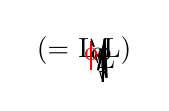
\begin{tikzpicture}[xscale=\myscalex-0.05,yscale=\myscaley-0.05]
\node (tone) at (5.2,0) {(= L.L)};
\node (syl) at (0,0) {\textsigma};
\node (syl3) at (3.4,0) {\red{\textsigma}};
\node (Rt) at (0,1) {o};
\node (Rt2) at (1.7,1) {o};
\node (Rt3) at (3.4,1) {\red{o}};
\node (H) at (-0.5,2) {L};
\node (R) at (0.5,3) {l};
\draw [thick] (syl.north) -- (Rt.south) ;
\draw [thick] (syl.north) -- (Rt2.south) ;
\draw [thick,red] (syl3.north) -- (Rt3.south) ;
\draw [thick] (Rt.north) -- (H.south) ;
\draw [thick] (Rt.north) -- (R.south) ;
\draw [dashed] (Rt3.north) -- (H.south) ;
\draw [dashed] (Rt3.north) -- (R.south) ;
\end{tikzpicture}
\end{minipage}
}  
  
\newcommand{\ilit}[1]{#1\il{#1}}    
\newcommand{\isit}[1]{#1\is{#1}}  

\makeatletter
\let\thetitle\@title
\let\theauthor\@author 
\makeatother

\newcommand{\togglepaper}[1][0]{ 
  \bibliography{../localbibliography}
  %% hyphenation points for line breaks
%% Normally, automatic hyphenation in LaTeX is very good
%% If a word is mis-hyphenated, add it to this file
%%
%% add information to TeX file before \begin{document} with:
%% %% hyphenation points for line breaks
%% Normally, automatic hyphenation in LaTeX is very good
%% If a word is mis-hyphenated, add it to this file
%%
%% add information to TeX file before \begin{document} with:
%% \include{localhyphenation}
\hyphenation{
affri-ca-te
affri-ca-tes
com-ple-ments
par-a-digm
Sha-ron
Kings-ton
phe-nom-e-non
Daul-ton
Abu-ba-ka-ri
Ngo-nya-ni
Clem-ents 
King-ston
Tru-cken-brodt
Tab-leau
cophono-logies
mark-edness
Ti-gri-nya
a-mong
Car-stens
Lu-bu-ku-su
}
\hyphenation{
affri-ca-te
affri-ca-tes
com-ple-ments
par-a-digm
Sha-ron
Kings-ton
phe-nom-e-non
Daul-ton
Abu-ba-ka-ri
Ngo-nya-ni
Clem-ents 
King-ston
Tru-cken-brodt
Tab-leau
cophono-logies
mark-edness
Ti-gri-nya
a-mong
Car-stens
Lu-bu-ku-su
}
  \papernote{\scriptsize\normalfont
    \theauthor.
    \thetitle. 
    To appear in: 
    Emily Clem,   Peter Jenks \& Hannah Sande.
    Theory and description in African Linguistics: Selected papers from the 47th Annual Conference on African Linguistics.
    Berlin: Language Science Press. [preliminary page numbering]
  }
  \pagenumbering{roman}
  \setcounter{chapter}{#1}
  \addtocounter{chapter}{-1}
}

\newcommand{\upstep}{\textupstep}


% \newcounter{tableauxcounter}

\renewcommand{\textltailn}{ɲ}
\renewcommand{\textbardotlessj}{ɟ}

\newcommand{\emphkh}[1]{\textit{#1}} %originally \textbf, banned by the guidelines



\definecolor{lsDOIGray}{cmyk}{0,0,0,0.45}


\newcommand{\xuparrow}[1]{%
  {\left\uparrow\vbox to #1{}\right.\kern-\nulldelimiterspace}
}
\renewcommand \textupstep[1]{\char"A71B#1}
\renewcommand \textdownstep[1]{\char"A71C#1}
 
 \newcommand{\ꜛ}{\textsf{ꜛ}}
 
\def\biberror{\undefined}


\newcommand{\OTbox}[1]{\resizebox{.88\textwidth}{!}{#1}}
 
% \usepackage{pifont.sty}

\author{Laura Downing\affiliation{University of Gothenburg}}
\title{Tumbuka prosody: Between tone and stress}
\abstract{Tumbuka is spoken in the northern Lake Malawi region where it is typical for Bantu languages to have what has been called a restricted tone system: all words must have a High tone. This kind of prosodic system has stress-like properties, and functions similar to \citet{Kisseberth&Odden2003}. \citet{Vail1972} suggests that Tumbuka is a purely stress language. This paper argues, in contrast, that because Tumbuka High tone realization has tone-like properties, as defined in \citet{Hyman2006,Hyman2009,Hyman2012,Hyman2014}, as well as stress-like properties, it cannot be considered a canonical stress language. It is proposed that the synchronic Tumbuka prosodic system evolved from one where contrastive High tone takes a phrasal domain through processes – formalizable as an OT factorial typology – which made phrasal prosody more transparently predictable by eliminating most tonal contrasts.}

\IfFileExists{../localcommands.tex}{%hack to check whether this is being compiled as part of a collection or standalone
  \usepackage{pifont}
\usepackage{savesym}

\savesymbol{downingtriple}
\savesymbol{downingdouble}
\savesymbol{downingquad}
\savesymbol{downingquint}
\savesymbol{suph}
\savesymbol{supj}
\savesymbol{supw}
\savesymbol{sups}
\savesymbol{ts}
\savesymbol{tS}
\savesymbol{devi}
\savesymbol{devu}
\savesymbol{devy}
\savesymbol{deva}
\savesymbol{N}
\savesymbol{Z}
\savesymbol{circled}
\savesymbol{sem}
\savesymbol{row}
\savesymbol{tipa}
\savesymbol{tableauxcounter}
\savesymbol{tabhead}
\savesymbol{inp}
\savesymbol{inpno}
\savesymbol{g}
\savesymbol{hanl}
\savesymbol{hanr}
\savesymbol{kuku}
\savesymbol{ip}
\savesymbol{lipm}
\savesymbol{ripm}
\savesymbol{lipn}
\savesymbol{ripn} 
% \usepackage{amsmath} 
% \usepackage{multicol}
\usepackage{qtree} 
\usepackage{tikz-qtree,tikz-qtree-compat}
% \usepackage{tikz}
\usepackage{upgreek}


%%%%%%%%%%%%%%%%%%%%%%%%%%%%%%%%%%%%%%%%%%%%%%%%%%%%
%%%                                              %%%
%%%           Examples                           %%%
%%%                                              %%%
%%%%%%%%%%%%%%%%%%%%%%%%%%%%%%%%%%%%%%%%%%%%%%%%%%%%
% remove the percentage signs in the following lines
% if your book makes use of linguistic examples
\usepackage{tipa}  
\usepackage{pstricks,pst-xkey,pst-asr}

%for sande et al
\usepackage{pst-jtree}
\usepackage{pst-node}
%\usepackage{savesym}


% \usepackage{subcaption}
\usepackage{multirow}  
\usepackage{./langsci/styles/langsci-optional} 
\usepackage{./langsci/styles/langsci-lgr} 
\usepackage{./langsci/styles/langsci-glyphs} 
\usepackage[normalem]{ulem}
%% if you want the source line of examples to be in italics, uncomment the following line
% \def\exfont{\it}
\usetikzlibrary{arrows.meta,topaths,trees}
\usepackage[linguistics]{forest}
\forestset{
	fairly nice empty nodes/.style={
		delay={where content={}{shape=coordinate,for parent={
					for children={anchor=north}}}{}}
}}
\usepackage{soul}
\usepackage{arydshln}
% \usepackage{subfloat}
\usepackage{langsci/styles/langsci-gb4e} 
   
% \usepackage{linguex}
\usepackage{vowel}

\usepackage{pifont}% http://ctan.org/pkg/pifont
\newcommand{\cmark}{\ding{51}}%
\newcommand{\xmark}{\ding{55}}%
 
 
 %Lamont
 \makeatletter
\g@addto@macro\@floatboxreset\centering
\makeatother

\usepackage{newfloat} 
\DeclareFloatingEnvironment[fileext=tbx,name=Tableau]{tableau}
  %add all your local new commands to this file
\newcommand{\downingquad}[4]{\parbox{2.5cm}{#1}\parbox{3.5cm}{#2}\parbox{2.5cm}{#3}\parbox{3.5cm}{#4}}
\newcommand{\downingtriple}[3]{\parbox{4.5cm}{#1}\parbox{3cm}{#2}\parbox{3cm}{#3}}
\newcommand{\downingdouble}[2]{\parbox{4.5cm}{#1}\parbox{6cm}{#2}}
\newcommand{\downingquint}[5]{\parbox{1.75cm}{#1}\parbox{2.25cm}{#2}\parbox{2cm}{#3}\parbox{3cm}{#4}\parbox{2cm}{#5}}
\newcolumntype{Y}{>{\centering\arraybackslash}X}
\newcolumntype{T}{>{\centering\arraybackslash}m{2cm}}

%commands for Kusmer paper below
\newcommand{\ip}{$\upiota$}
\newcommand{\lipm}{(\_{\ip-Max}}
\newcommand{\ripm}{)\_{\ip-Max}}
\newcommand{\lipn}{(\_{\ip}}
\newcommand{\ripn}{)\_{\ip}}
\renewcommand{\_}[1]{\textsubscript{#1}}


%commands for Pillion paper below
\newcommand{\suph}{\textipa{\super h}}
\newcommand{\supj}{\textipa{\super j}}
\newcommand{\supw}{\textipa{\super w}}
\newcommand{\ts}{\textipa{\t{ts}}}
\newcommand{\tS}{\textipa{\t{tS}}}
\newcommand{\devi}{\textipa{\r*i}}
\newcommand{\devu}{\textipa{\r*u}}
\newcommand{\devy}{\textipa{\r*y}}
\newcommand{\deva}{\textipa{\r*a}}
\renewcommand{\N}{\textipa{N}}
\newcommand{\Z}{\textipa{Z}}
% 

%commands for Diercks paper below
\newcommand{\circled}[1]{\begin{tikzpicture}[baseline=(word.base)]
\node[draw, rounded corners, text height=8pt, text depth=2pt, inner sep=2pt, outer sep=0pt, use as bounding box] (word) {#1};
\end{tikzpicture}
}

%commands for Pesetsky paper below
% \newcommand{\sem}[2][]{\mbox{$[\![ $\textbf{#2}$ ]\!]^{#1}$}}
\newcommand{\sem}[2][]{\mbox{$[[ $\textbf{#2}$ ]]^{#1}$}}

% \newcommand{\ripn}{{\color{red}ripn}}%this is used but never defined. Please update the definition



%commands for Lamont paper below
\newcommand{\row}[4]{
	#1. & 
    /{#2}/ & 
    [{#3}] & 
    `#4' \\ 
}
%\newcounter{tableauxcounter}
\newcommand{\tabhead}[2]{
%     \captionsetup{labelformat=empty}
%     \stepcounter{tableauxcounter}
%     \addtocounter{table}{-1}
% 	\centering
% 	\caption{Tableau \thetableauxcounter: #1}
	\caption{#1}
	\label{#2}
}
\newcommand{\candref}[2]{{(\ref{#1}#2)}}
\newcommand{\tableauref}[1]{{Tableau~\ref{#1}}}
% tableaux
\newcommand{\inp}[1]{\multicolumn{2}{|l||}{{#1}}}
\newcommand{\inpno}[1]{\multicolumn{2}{|l||}{#1}}
\newcommand{\g}{\cellcolor{lightgray}}
\newcommand{\hanl}{\HandLeft}
\newcommand{\hanr}{\HandRight}
\newcommand{\kuku}{Kuk\'{u}}

% \newcommand{\nocaption}[1]{{\color{red} Please provide a caption}}

% \providecommand{\biberror}[1]{{\color{red}#1}}

\definecolor{RED}{cmyk}{0.05,1,0.8,0}


\newfontfamily\amharicfont[Script = Ethiopic, Scale = 1.0]{AbyssinicaSIL}
\newcommand{\amh}[1]{{\amharicfont #1}}

% 
% %Gjersoe
\usepackage{textgreek}
% 
\newcommand{\viol}{\fontfamily{MinionPro-OsF}\selectfont\rotatebox{60}{$\star$}}
\newcommand{\myscalex}{0.45}
\newcommand{\myscaley}{0.65}
%\newcommand{\red}[1]{\textcolor{red}{#1}}
%\newcommand{\blue}[1]{\textcolor{blue}{#1}}
\newcommand{\epen}[1]{\colorbox{jgray}{#1}}
\newcommand{\hand}{{\normalsize \ding{43}}}
\definecolor{jgray}{gray}{0.8} 
\usetikzlibrary{positioning}
\usetikzlibrary{matrix}
\newcommand{\mora}{\textmu\xspace}
\newcommand{\si}{\textsigma\xspace}
\newcommand{\ft}{\textPhi\xspace}
\newcommand{\tone}{\texttau\xspace}
\newcommand{\word}{\textomega\xspace}
% \newcommand{\ts}{\texttslig}
\newcommand{\fns}{\footnotesize}
\newcommand{\ns}{\normalsize}
\newcommand{\vs}{\vspace{1em}}
\newcommand{\bs}{\textbackslash}   % backslash
\newcommand{\cmd}[1]{{\bf \color{red}#1}}   % highlights command
\newcommand{\scell}[2][l]{\begin{tabular}[#1]{@{}c@{}}#2\end{tabular}}
% \interfootnotelinepenalty=10000

% --- Snider Representations --- %

\newcommand{\RepLevelHh}{
\begin{minipage}{0.10\textwidth}
\begin{tikzpicture}[xscale=\myscalex,yscale=\myscaley]
%\node (syl) at (0,0) {Hi};
\node (Rt) at (0,1) {o};
\node (H) at (-0.5,2) {H};
\node (R) at (0.5,3) {h};
%\draw [thick] (syl.north) -- (Rt.south) ;
\draw [thick] (Rt.north) -- (H.south) ;
\draw [thick] (Rt.north) -- (R.south) ;
\end{tikzpicture}
\end{minipage}
}

\newcommand{\RepLevelLh}{
\begin{minipage}{0.10\textwidth}
\begin{tikzpicture}[xscale=\myscalex,yscale=\myscaley]
%\node (syl) at (0,0) {Mid2};
\node (Rt) at (0,1) {o};
\node (H) at (-0.5,2) {L};
\node (R) at (0.5,3) {h};
%\draw [thick] (syl.north) -- (Rt.south) ;
\draw [thick] (Rt.north) -- (H.south) ;
\draw [thick] (Rt.north) -- (R.south) ;
\end{tikzpicture}
\end{minipage}
}

\newcommand{\RepLevelHl}{
\begin{minipage}{0.10\textwidth}
\begin{tikzpicture}[xscale=\myscalex,yscale=\myscaley]
%\node (syl) at (0,0) {Mid1};
\node (Rt) at (0,1) {o};
\node (H) at (-0.5,2) {H};
\node (R) at (0.5,3) {l};
%\draw [thick] (syl.north) -- (Rt.south) ;
\draw [thick] (Rt.north) -- (H.south) ;
\draw [thick] (Rt.north) -- (R.south) ;
\end{tikzpicture}
\end{minipage}
}

\newcommand{\RepLevelLl}{
\begin{minipage}{0.10\textwidth}
\begin{tikzpicture}[xscale=\myscalex,yscale=\myscaley]
%\node (syl) at (0,0) {Lo};
\node (Rt) at (0,1) {o};
\node (H) at (-0.5,2) {L};
\node (R) at (0.5,3) {l};
%\draw [thick] (syl.north) -- (Rt.south) ;
\draw [thick] (Rt.north) -- (H.south) ;
\draw [thick] (Rt.north) -- (R.south) ;
\end{tikzpicture}
\end{minipage}
}

% --- Representations --- %

\newcommand{\RepLevel}{
\begin{minipage}{0.10\textwidth}
\begin{tikzpicture}[xscale=\myscalex,yscale=\myscaley]
\node (syl) at (0,0) {\textsigma};
\node (Rt) at (0,1) {o};
\node (H) at (-0.5,2) {\texttau};
\node (R) at (0.5,3) {\textrho};
\draw [thick] (syl.north) -- (Rt.south) ;
\draw [thick] (Rt.north) -- (H.south) ;
\draw [thick] (Rt.north) -- (R.south) ;
\end{tikzpicture}
\end{minipage}
}

\newcommand{\RepContour}{
\begin{minipage}{0.10\textwidth}
\begin{tikzpicture}[xscale=\myscalex,yscale=\myscaley]
\node (syl) at (0,0) {\textsigma};
\node (Rt) at (0,1) {o};
\node (H) at (-0.5,2) {\texttau};
\node (R) at (0.5,3) {\textrho};
\node (Rt2) at (1.5,1.0) {o};
%\node (H2) at (1.0,2) {$\tau$};
%\node (R2) at (2.0,2.5) {R};
\draw [thick] (syl.north) -- (Rt.south) ;
\draw [thick] (Rt.north) -- (H.south) ;
\draw [thick] (Rt.north) -- (R.south) ;
\draw [thick] (syl.north) -- (Rt2.south) ;
%\draw [thick] (Rt2.north) -- (H2.south) ;
%\draw [thick] (Rt2.north) -- (R2.south) ;
\end{tikzpicture}
\end{minipage}
}


% --- OT constraints --- %

\newcommand{\IllustrationDown}{
\begin{minipage}{0.09\textwidth}
\begin{tikzpicture}[xscale=0.7,yscale=0.45]
\node (reg) at (0,0.75) {{\small \textalpha}};
\node (arrow) at (0,0) {{\fns $\downarrow$}};
\node (Rt) at (0,-0.75) {{\small \textbeta}};
\end{tikzpicture}
\end{minipage}
}

\newcommand{\IllustrationUp}{
\begin{minipage}{0.09\textwidth}
\begin{tikzpicture}[xscale=0.7,yscale=0.45]
\node (reg) at (0,0.75) {{\small \textalpha}};
\node (arrow) at (0,0) {{\fns $\uparrow$}};
\node (Rt) at (0,-0.75) {{\small \textbeta}};
\end{tikzpicture}
\end{minipage}
}

\newcommand{\MaxAB}{
\begin{minipage}{0.09\textwidth}
\begin{tikzpicture}[xscale=0.6,yscale=0.4]
\node (max) at (0,0) {{\small \textsc{Max}}};
\node (reg) at (0.75,0.5) {{\fns \textalpha}};
\node (arrow) at (0.75,0) {{\tiny $\downarrow$}};
\node (Rt) at (0.75,-0.5) {{\fns \textbeta}};
\end{tikzpicture}
\end{minipage}
}

\newcommand{\DepAB}{
\begin{minipage}{0.09\textwidth}
\begin{tikzpicture}[xscale=0.6,yscale=0.4]
\node (max) at (0,0) {{\small \textsc{Dep}}};
\node (reg) at (0.75,0.5) {{\fns \textalpha}};
\node (arrow) at (0.75,0) {{\tiny $\downarrow$}};
\node (Rt) at (0.75,-0.5) {{\fns \textbeta}};
\end{tikzpicture}
\end{minipage}
}

\newcommand{\DepHReg}{
\begin{minipage}{0.055\textwidth}
\begin{tikzpicture}[xscale=0.6,yscale=0.4]
\node (dep) at (0,0) {{\small \textsc{Dep}}};
\node (reg) at (0,-1.0) {{\small h}};
\end{tikzpicture}
\end{minipage}
}

\newcommand{\DepLReg}{
\begin{minipage}{0.055\textwidth}
\begin{tikzpicture}[xscale=0.6,yscale=0.4]
\node (dep) at (0,0) {{\small \textsc{Dep}}};
\node (reg) at (0,-1.0) {{\small l}};
\end{tikzpicture}
\end{minipage}
}

\newcommand{\DepReg}{
\begin{minipage}{0.055\textwidth}
\begin{tikzpicture}[xscale=0.6,yscale=0.4]
\node (dep) at (0,0) {{\small \textsc{Dep}}};
\node (reg) at (0,-1.0) {{\small \textrho}};
\end{tikzpicture}
\end{minipage}
}

\newcommand{\DepTRt}{
\begin{minipage}{0.1\textwidth}
\begin{tikzpicture}[xscale=0.6,yscale=0.4]
\node (dep) at (0,0) {{\small \textsc{Dep}}};
\node (t) at (0.75,0.5) {{\fns \texttau}};
\node (arrow) at (0.75,0) {{\tiny $\downarrow$}};
\node (Rt) at (0.75,-0.5) {{\fns o}};
\end{tikzpicture}
\end{minipage}
}

\newcommand{\MaxRegRt}{
\begin{minipage}{0.1\textwidth}
\begin{tikzpicture}[xscale=0.6,yscale=0.4]
\node (max) at (0,0) {{\small \textsc{Max}}};
\node (arrow) at (0.75,0) {{\tiny $\downarrow$}};
\node (Rt) at (0.75,-0.5) {{\fns o}};
\node (reg) at (0.75,0.5) {{\fns \textrho}};
\end{tikzpicture}
\end{minipage}
}

\newcommand{\RegToneByRt}{
\begin{minipage}{0.06\textwidth}
\begin{tikzpicture}[xscale=0.6,yscale=0.5]
\node[rotate=20] (arrow1) at (-0.15,0) {{\fns $\uparrow$}};
\node[rotate=340] (arrow2) at (0.15,0) {{\fns $\uparrow$}};
\node (Rt) at (0,-0.55) {{\small o}};
\node (reg) at (0.4,0.55) {{\small \textrho}};
\node (tone) at (-0.4,0.55) {{\small \texttau}};
\end{tikzpicture}
\end{minipage}
}

\newcommand{\RegToneBySyl}{
\begin{minipage}{0.06\textwidth}
\begin{tikzpicture}[xscale=0.6,yscale=0.5]
\node[rotate=20] (arrow1) at (-0.15,0) {{\fns $\uparrow$}};
\node[rotate=340] (arrow2) at (0.15,0) {{\fns $\uparrow$}};
\node (Rt) at (0,-0.55) {{\small \textsigma}};
\node (reg) at (0.4,0.55) {{\small \textrho}};
\node (tone) at (-0.4,0.55) {{\small \texttau}};
\end{tikzpicture}
\end{minipage}
}

\newcommand{\DepTone}{
\begin{minipage}{0.055\textwidth}
\begin{tikzpicture}[xscale=0.6,yscale=0.4]
\node (dep) at (0,0) {{\small \textsc{Dep}}};
\node (tone) at (0,-1.0) {{\small \texttau}};
\end{tikzpicture}
\end{minipage}
}

\newcommand{\DepTonalRt}{
\begin{minipage}{0.055\textwidth}
\begin{tikzpicture}[xscale=0.6,yscale=0.4]
\node (dep) at (0,0) {{\small \textsc{Dep}}};
\node (tone) at (0,-1.0) {{\small o}};
\end{tikzpicture}
\end{minipage}
}

\newcommand{\DepL}{
\begin{minipage}{0.055\textwidth}
\begin{tikzpicture}[xscale=0.6,yscale=0.4]
\node (dep) at (0,0) {{\small \textsc{Dep}}};
\node (tone) at (0,-1.0) {{\small L}};
\end{tikzpicture}
\end{minipage}
}

\newcommand{\DepH}{
\begin{minipage}{0.055\textwidth}
\begin{tikzpicture}[xscale=0.6,yscale=0.4]
\node (dep) at (0,0) {{\small \textsc{Dep}}};
\node (tone) at (0,-1.0) {{\small H}};
\end{tikzpicture}
\end{minipage}
}

\newcommand{\NoMultDiff}{{\small *loh}}
\newcommand{\Alt}{{\small \textsc{Alt}}}
\newcommand{\NoSkip}{{\small \scell{\textsc{No}\\\textsc{Skip}}}}


\newcommand{\RegDomRt}{
\begin{minipage}{0.030\textwidth}
\begin{tikzpicture}[xscale=0.6,yscale=0.5]
\node (arrow) at (0,0) {{\fns $\downarrow$}};
\node (Rt) at (0,-0.55) {{\small o}};
\node (reg) at (0,0.55) {{\small \textrho}};
\end{tikzpicture}
\end{minipage}
}

\newcommand{\DepRegRt}{
\begin{minipage}{0.1\textwidth}
\begin{tikzpicture}[xscale=0.6,yscale=0.4]
\node (dep) at (0,0) {{\small \textsc{Dep}}};
\node (arrow) at (0.75,0) {{\tiny $\downarrow$}};
\node (Rt) at (0.75,-0.5) {{\fns o}};
\node (reg) at (0.75,0.5) {{\fns \textrho}};
\end{tikzpicture}
\end{minipage}
}

% unused

\newcommand{\ToneByRt}{
\begin{minipage}{0.05\textwidth}
\begin{tikzpicture}[xscale=0.6,yscale=0.5]
\node (arrow) at (0,0) {{\fns $\uparrow$}};
\node (Rt) at (0,-0.55) {{\small o}};
\node (tone) at (0,0.55) {{\small \texttau}};
\end{tikzpicture}
\end{minipage}
}

\newcommand{\RegByRt}{
\begin{minipage}{0.05\textwidth}
\begin{tikzpicture}[xscale=0.6,yscale=0.5]
\node (arrow) at (0,0) {{\fns $\uparrow$}};
\node (Rt) at (0,-0.55) {{\small o}};
\node (reg) at (0,0.55) {{\small \textrho}};
\end{tikzpicture}
\end{minipage}
}

\newcommand{\ToneDomRt}{
\begin{minipage}{0.05\textwidth}
\begin{tikzpicture}[xscale=0.6,yscale=0.5]
\node (arrow) at (0,0) {{\fns $\downarrow$}};
\node (Rt) at (0,-0.55) {{\small o}};
\node (tone) at (0,0.55) {{\small \texttau}};
\end{tikzpicture}
\end{minipage}
}

% --- OT tableaus --- %

% Sec. 3.2, first tabl.

\newcommand{\OTHLInput}{
\begin{minipage}{0.17\textwidth}
\begin{tikzpicture}[xscale=\myscalex,yscale=\myscaley]
\node (tone) at (2,0) {(= H)};
\node (syl) at (0,0) {\textsigma};
\node (Rt) at (0,1) {o};
\node (H) at (-0.5,2) {H};
\node (R) at (0.5,3) {h};
\node (Rt2) at (1.5,1.0) {o};
%\node (H2) at (1.0,2) {\epen{L}};
\node (R2) at (2.0,3) {\blue{l}};
\draw [thick] (syl.north) -- (Rt.south) ;
\draw [thick] (Rt.north) -- (H.south) ;
\draw [thick] (Rt.north) -- (R.south) ;
\draw [thick] (syl.north) -- (Rt2.south) ;
%\draw [dashed] (Rt2.north) -- (H2.south) ;
%\draw [dashed] (Rt2.north) -- (R2.south) ;
\end{tikzpicture}
\end{minipage}
}

\newcommand{\OTHLWinner}{
\begin{minipage}{0.17\textwidth}
\begin{tikzpicture}[xscale=\myscalex,yscale=\myscaley]
\node (tone) at (2,0) {(= HL)};
\node (syl) at (0,0) {\textsigma};
\node (Rt) at (0,1) {o};
\node (H) at (-0.5,2) {H};
\node (R) at (0.5,3) {h};
\node (Rt2) at (1.5,1.0) {o};
\node (H2) at (1.0,2) {\epen{L}};
\node (R2) at (2.0,3) {\blue{l}};
\draw [thick] (syl.north) -- (Rt.south) ;
\draw [thick] (Rt.north) -- (H.south) ;
\draw [thick] (Rt.north) -- (R.south) ;
\draw [thick] (syl.north) -- (Rt2.south) ;
\draw [dashed] (Rt2.north) -- (H2.south) ;
\draw [dashed] (Rt2.north) -- (R2.south) ;
\end{tikzpicture}
\end{minipage}
}

\newcommand{\OTHLSpreadingHOnly}{
\begin{minipage}{0.17\textwidth}
\begin{tikzpicture}[xscale=\myscalex,yscale=\myscaley]
\node (tone) at (2,0) {(= HM)};
\node (syl) at (0,0) {\textsigma};
\node (Rt) at (0,1) {o};
\node (H) at (-0.5,2) {H};
\node (R) at (0.5,3) {h};
\node (Rt2) at (1.5,1.0) {o};
%\node (H2) at (1.0,2) {\epen{L}};
\node (R2) at (2.0,3) {\blue{l}};
\draw [thick] (syl.north) -- (Rt.south) ;
\draw [thick] (Rt.north) -- (H.south) ;
\draw [thick] (Rt.north) -- (R.south) ;
\draw [thick] (syl.north) -- (Rt2.south) ;
\draw [dashed] (Rt2.north) -- (R2.south) ;
\draw [dashed] (Rt2.north) -- (H.south) ;
\end{tikzpicture}
\end{minipage}
}

\newcommand{\OTHLInsertH}{
\begin{minipage}{0.17\textwidth}
\begin{tikzpicture}[xscale=\myscalex,yscale=\myscaley]
\node (tone) at (2,0) {(= HM)};
\node (syl) at (0,0) {\textsigma};
\node (Rt) at (0,1) {o};
\node (H) at (-0.5,2) {H};
\node (R) at (0.5,3) {h};
\node (Rt2) at (1.5,1.0) {o};
\node (H2) at (1.0,2) {\epen{H}};
\node (R2) at (2.0,3) {\blue{l}};
\draw [thick] (syl.north) -- (Rt.south) ;
\draw [thick] (Rt.north) -- (H.south) ;
\draw [thick] (Rt.north) -- (R.south) ;
\draw [thick] (syl.north) -- (Rt2.south) ;
\draw [dashed] (Rt2.north) -- (H2.south) ;
\draw [dashed] (Rt2.north) -- (R2.south) ;
\end{tikzpicture}
\end{minipage}
}

\newcommand{\OTHLOverwriting}{
\begin{minipage}{0.17\textwidth}
\begin{tikzpicture}[xscale=\myscalex,yscale=\myscaley]
\node (syl) at (0,0) {\textsigma};
\node (Rt) at (0,1) {o};
\node (H) at (-0.5,2) {H};
\node (R) at (0.5,3) {h};
\node (Rt2) at (1.5,1.0) {o};
%\node (H2) at (1.0,2) {\epen{L}};
\node (R2) at (2.0,3) {\blue{l}};
\draw [thick] (syl.north) -- (Rt.south) ;
\draw [thick] (Rt.north) -- (H.south) ;
\draw [thick] (Rt.north) -- (R.south) ;
\draw [thick] (syl.north) -- (Rt2.south) ;
%\draw [dashed] (Rt2.north) -- (H2.south) ;
\draw [dashed] (Rt.north) -- (R2.south) ;
\node (del) at (0.3,1.9) {\textbf{=}};
\end{tikzpicture}
\end{minipage}
}

\newcommand{\OTHLSpreading}{
\begin{minipage}{0.17\textwidth}
\begin{tikzpicture}[xscale=\myscalex,yscale=\myscaley]
\node (syl) at (0,0) {\textsigma};
\node (Rt) at (0,1) {o};
\node (H) at (-0.5,2) {H};
\node (R) at (0.5,3) {h};
\node (Rt2) at (1.5,1.0) {o};
%\node (H2) at (1.0,2) {\epen{L}};
\node (R2) at (2.0,3) {\blue{l}};
\draw [thick] (syl.north) -- (Rt.south) ;
\draw [thick] (Rt.north) -- (H.south) ;
\draw [thick] (Rt.north) -- (R.south) ;
\draw [thick] (syl.north) -- (Rt2.south) ;
%\draw [dashed] (Rt2.north) -- (H2.south) ;
\draw [dashed] (Rt2.north) -- (H.south) ;
\draw [dashed] (Rt2.north) -- (R.south) ;
\end{tikzpicture}
\end{minipage}
}

% Sec. 4.2, second tabl.: phrase-medial position

\newcommand{\OTHnoLInput}{
\begin{minipage}{0.17\textwidth}
\begin{tikzpicture}[xscale=\myscalex,yscale=\myscaley]
\node (tone) at (2,0) {(= H)};
\node (syl) at (0,0) {\textsigma};
\node (Rt) at (0,1) {o};
\node (H) at (-0.5,2) {H};
\node (R) at (0.5,3) {h};
\node (Rt2) at (1.5,1.0) {o};
%\node (H2) at (1.0,2) {\epen{L}};
%\node (R2) at (2.0,3) {\blue{l}};
\draw [thick] (syl.north) -- (Rt.south) ;
\draw [thick] (Rt.north) -- (H.south) ;
\draw [thick] (Rt.north) -- (R.south) ;
\draw [thick] (syl.north) -- (Rt2.south) ;
\end{tikzpicture}
\end{minipage}
}

\newcommand{\OTHnoLEpenth}{
\begin{minipage}{0.17\textwidth}
\begin{tikzpicture}[xscale=\myscalex,yscale=\myscaley]
\node (tone) at (2,0) {(= HM)};
\node (syl) at (0,0) {\textsigma};
\node (Rt) at (0,1) {o};
\node (H) at (-0.5,2) {H};
\node (R) at (0.5,3) {h};
\node (Rt2) at (1.5,1.0) {o};
\node (H2) at (1.0,2) {\epen{L}};
\node (R2) at (2.0,3) {\epen{h}};
\draw [thick] (syl.north) -- (Rt.south) ;
\draw [thick] (Rt.north) -- (H.south) ;
\draw [thick] (Rt.north) -- (R.south) ;
\draw [thick] (syl.north) -- (Rt2.south) ;
\draw [dashed] (Rt2.north) -- (H2.south) ;
\draw [dashed] (Rt2.north) -- (R2.south) ;
\end{tikzpicture}
\end{minipage}
}

\newcommand{\OTHnoLSpreading}{
\begin{minipage}{0.17\textwidth}
\begin{tikzpicture}[xscale=\myscalex,yscale=\myscaley]
\node (tone) at (2,0) {(= HH)};
\node (syl) at (0,0) {\textsigma};
\node (Rt) at (0,1) {o};
\node (H) at (-0.5,2) {H};
\node (R) at (0.5,3) {h};
\node (Rt2) at (1.5,1.0) {o};
%\node (H2) at (1.0,2) {\epen{L}};
%\node (R2) at (2.0,3) {\blue{l}};
\draw [thick] (syl.north) -- (Rt.south) ;
\draw [thick] (Rt.north) -- (H.south) ;
\draw [thick] (Rt.north) -- (R.south) ;
\draw [thick] (syl.north) -- (Rt2.south) ;
\draw [dashed] (Rt2.north) -- (H.south) ;
\draw [dashed] (Rt2.north) -- (R.south) ;
\end{tikzpicture}
\end{minipage}
}

% Sec. 4.2, third tabl., LM is unaffected by L\%

\newcommand{\OTLMInput}{
\begin{minipage}{0.2\textwidth}
\begin{tikzpicture}[xscale=\myscalex,yscale=\myscaley]
\node (tone) at (2,0) {(= LM)};
\node (syl) at (0,0) {\textsigma};
\node (Rt) at (0,1) {o};
\node (H) at (-0.5,2) {L};
\node (R) at (0.5,3) {l};
\node (Rt2) at (1.5,1.0) {o};
\node (H2) at (1.0,2) {L};
\node (R2) at (2.0,3) {h};
\node (R3) at (3.0,3) {\blue{l}};
\draw [thick] (syl.north) -- (Rt.south) ;
\draw [thick] (Rt.north) -- (H.south) ;
\draw [thick] (Rt.north) -- (R.south) ;
\draw [thick] (syl.north) -- (Rt2.south) ;
\draw [thick] (Rt2.north) -- (H2.south) ;
\draw [thick] (Rt2.north) -- (R2.south) ;
\end{tikzpicture}
\end{minipage}
}

\newcommand{\OTLMReplace}{
\begin{minipage}{0.2\textwidth}
\begin{tikzpicture}[xscale=\myscalex,yscale=\myscaley]
\node (tone) at (2,0) {(= LL)};
\node (syl) at (0,0) {\textsigma};
\node (Rt) at (0,1) {o};
\node (H) at (-0.5,2) {L};
\node (R) at (0.5,3) {l};
\node (Rt2) at (1.5,1.0) {o};
\node (H2) at (1.0,2) {L};
\node (R2) at (2.0,3) {h};
\node (R3) at (3.0,3) {\blue{l}};
\draw [thick] (syl.north) -- (Rt.south) ;
\draw [thick] (Rt.north) -- (H.south) ;
\draw [thick] (Rt.north) -- (R.south) ;
\draw [thick] (syl.north) -- (Rt2.south) ;
\draw [thick] (Rt2.north) -- (H2.south) ;
\draw [thick] (Rt2.north) -- (R2.south) ;
\draw [dashed] (Rt2.north) -- (R3.south) ;
\node (del) at (1.8,2.1) {\textbf{=}};
\end{tikzpicture}
\end{minipage}
}

\newcommand{\OTLMTwoReg}{
\begin{minipage}{0.2\textwidth}
\begin{tikzpicture}[xscale=\myscalex,yscale=\myscaley]
\node (tone) at (2,0) {(= LML)};
\node (syl) at (0,0) {\textsigma};
\node (Rt) at (0,1) {o};
\node (H) at (-0.5,2) {L};
\node (R) at (0.5,3) {l};
\node (Rt2) at (1.5,1.0) {o};
\node (H2) at (1.0,2) {L};
\node (R2) at (2.0,3) {h};
\node (R3) at (3.0,3) {\blue{l}};
\draw [thick] (syl.north) -- (Rt.south) ;
\draw [thick] (Rt.north) -- (H.south) ;
\draw [thick] (Rt.north) -- (R.south) ;
\draw [thick] (syl.north) -- (Rt2.south) ;
\draw [thick] (Rt2.north) -- (H2.south) ;
\draw [thick] (Rt2.north) -- (R2.south) ;
\draw [dashed] (Rt2.north) -- (R3.south) ;
\end{tikzpicture}
\end{minipage}
}

% Sec. 4.2, fourth tabl., L is affected by L\% but M is not

\newcommand{\OTLInput}{
\begin{minipage}{0.17\textwidth}
\begin{tikzpicture}[xscale=\myscalex,yscale=\myscaley]
\node (tone) at (2,0) {(= L)};
\node (syl) at (0,0) {\textsigma};
\node (Rt) at (0,1) {o};
\node (H) at (-0.5,2) {L};
\node (R) at (0.5,3) {l};
\node (R2) at (2,3) {\blue{l}};
\draw [thick] (syl.north) -- (Rt.south) ;
\draw [thick] (Rt.north) -- (H.south) ;
\draw [thick] (Rt.north) -- (R.south) ;
\end{tikzpicture}
\end{minipage}
}

\newcommand{\OTLLowered}{
\begin{minipage}{0.17\textwidth}
\begin{tikzpicture}[xscale=\myscalex,yscale=\myscaley]
\node (tone) at (2,0) {(= LL)};
\node (syl) at (0,0) {\textsigma};
\node (Rt) at (0,1) {o};
\node (H) at (-0.5,2) {L};
\node (R) at (0.5,3) {l};
\node (R2) at (2,3) {\blue{l}};
\draw [thick] (syl.north) -- (Rt.south) ;
\draw [thick] (Rt.north) -- (H.south) ;
\draw [thick] (Rt.north) -- (R.south) ;
\draw [dashed] (Rt.north) -- (R2.south) ;
\end{tikzpicture}
\end{minipage}
}

\newcommand{\OTMInput}{
\begin{minipage}{0.17\textwidth}
\begin{tikzpicture}[xscale=\myscalex,yscale=\myscaley]
\node (tone) at (2,0) {(= M)};
\node (syl) at (0,0) {\textsigma};
\node (Rt) at (0,1) {o};
\node (H) at (-0.5,2) {L};
\node (R) at (0.5,3) {h};
\node (R2) at (2,3) {\blue{l}};
\draw [thick] (syl.north) -- (Rt.south) ;
\draw [thick] (Rt.north) -- (H.south) ;
\draw [thick] (Rt.north) -- (R.south) ;
\end{tikzpicture}
\end{minipage}
}

\newcommand{\OTMLowered}{
\begin{minipage}{0.17\textwidth}
\begin{tikzpicture}[xscale=\myscalex,yscale=\myscaley]
\node (tone) at (2,0) {(= ML)};
\node (syl) at (0,0) {\textsigma};
\node (Rt) at (0,1) {o};
\node (H) at (-0.5,2) {L};
\node (R) at (0.5,3) {h};
\node (R2) at (2,3) {\blue{l}};
\draw [thick] (syl.north) -- (Rt.south) ;
\draw [thick] (Rt.north) -- (H.south) ;
\draw [thick] (Rt.north) -- (R.south) ;
\draw [dashed] (Rt.north) -- (R2.south) ;
\end{tikzpicture}
\end{minipage}
}

% Sec. 4.2, fifth tableau, polar questions with level tones

\newcommand{\OTLPolIn}{
\begin{minipage}{0.20\textwidth}
\begin{tikzpicture}[xscale=\myscalex-0.05,yscale=\myscaley-0.05]
\node (tone) at (3.5,0) {(= L)};
\node (syl) at (0,0) {\textsigma};
\node (syl2) at (2,0) {\red{\textsigma}};
\node (Rt) at (0,1) {o};
\node (H) at (-0.5,2) {L};
\node (R) at (0.5,3) {l};
\node (Rt2) at (2,1) {\red{o}};
\draw [thick] (syl.north) -- (Rt.south) ;
\draw [thick,red] (syl2.north) -- (Rt2.south) ;
\draw [thick] (Rt.north) -- (H.south) ;
\draw [thick] (Rt.north) -- (R.south) ;
\end{tikzpicture}
\end{minipage}
}

\newcommand{\OTLPolDef}{
\begin{minipage}{0.20\textwidth}
\begin{tikzpicture}[xscale=\myscalex-0.05,yscale=\myscaley-0.05]
\node (tone) at (3.5,0) {(= L.M)};
\node (syl) at (0,0) {\textsigma};
\node (syl2) at (2,0) {\red{\textsigma}};
\node (Rt) at (0,1) {o};
\node (H) at (-0.5,2) {L};
\node (R) at (0.5,3) {l};
\node (H2) at (1.5,2) {\epen{L}};
\node (R2) at (2.5,3) {\epen{h}};
\node (Rt2) at (2,1) {\red{o}};
\draw [thick] (syl.north) -- (Rt.south) ;
\draw [thick,red] (syl2.north) -- (Rt2.south) ;
\draw [thick] (Rt.north) -- (H.south) ;
\draw [thick] (Rt.north) -- (R.south) ;
\draw [semithick,dashed] (Rt2.north) -- (H2.south) ;
\draw [semithick,dashed] (Rt2.north) -- (R2.south) ;
\end{tikzpicture}
\end{minipage}
}

\newcommand{\OTLPolAlt}{
\begin{minipage}{0.20\textwidth}
\begin{tikzpicture}[xscale=\myscalex-0.05,yscale=\myscaley-0.05]
\node (tone) at (3.5,0) {(= L.L)};
\node (syl) at (0,0) {\textsigma};
\node (syl2) at (2,0) {\red{\textsigma}};
\node (Rt) at (0,1) {o};
\node (H) at (-0.5,2) {L};
\node (R) at (0.5,3) {l};
\node (Rt2) at (2,1) {\red{o}};
\draw [thick] (syl.north) -- (Rt.south) ;
\draw [thick,red] (syl2.north) -- (Rt2.south) ;
\draw [thick] (Rt.north) -- (H.south) ;
\draw [thick] (Rt.north) -- (R.south) ;
\draw [semithick,dashed] (Rt2.north) -- (H.south) ;
\draw [semithick,dashed] (Rt2.north) -- (R.south) ;
\end{tikzpicture}
\end{minipage}
}

% Sec. 4.2, sixth tableau, polar questions with contour tones

\newcommand{\OTLLPolIn}{
\begin{minipage}{0.23\textwidth}
\begin{tikzpicture}[xscale=\myscalex-0.05,yscale=\myscaley-0.05]
\node (tone) at (5.2,0) {(= L)};
\node (syl) at (0,0) {\textsigma};
\node (syl3) at (3.4,0) {\red{\textsigma}};
\node (Rt) at (0,1) {o};
\node (Rt2) at (1.7,1) {o};
\node (Rt3) at (3.4,1) {\red{o}};
\node (H) at (-0.5,2) {L};
\node (R) at (0.5,3) {l};
\draw [thick] (syl.north) -- (Rt.south) ;
\draw [thick] (syl.north) -- (Rt2.south) ;
\draw [thick,red] (syl3.north) -- (Rt3.south) ;
\draw [thick] (Rt.north) -- (H.south) ;
\draw [thick] (Rt.north) -- (R.south) ;
\end{tikzpicture}
\end{minipage}
}

\newcommand{\OTLLPolDef}{
\begin{minipage}{0.23\textwidth}
\begin{tikzpicture}[xscale=\myscalex-0.05,yscale=\myscaley-0.05]
\node (tone) at (5.2,0) {(= L.M)};
\node (syl) at (0,0) {\textsigma};
\node (syl3) at (3.4,0) {\red{\textsigma}};
\node (Rt) at (0,1) {o};
\node (Rt2) at (1.7,1) {o};
\node (Rt3) at (3.4,1) {\red{o}};
\node (H) at (-0.5,2) {L};
\node (R) at (0.5,3) {l};
\node (H3) at (2.9,2) {\epen{L}};
\node (R3) at (3.9,3) {\epen{h}};
\draw [thick] (syl.north) -- (Rt.south) ;
\draw [thick] (syl.north) -- (Rt2.south) ;
\draw [thick,red] (syl3.north) -- (Rt3.south) ;
\draw [thick] (Rt.north) -- (H.south) ;
\draw [thick] (Rt.north) -- (R.south) ;
\draw [dashed] (Rt3.north) -- (H3.south) ;
\draw [dashed] (Rt3.north) -- (R3.south) ;
\end{tikzpicture}
\end{minipage}
}

\newcommand{\OTLLPolSkip}{
\begin{minipage}{0.23\textwidth}
\begin{tikzpicture}[xscale=\myscalex-0.05,yscale=\myscaley-0.05]
\node (tone) at (5.2,0) {(= L.L)};
\node (syl) at (0,0) {\textsigma};
\node (syl3) at (3.4,0) {\red{\textsigma}};
\node (Rt) at (0,1) {o};
\node (Rt2) at (1.7,1) {o};
\node (Rt3) at (3.4,1) {\red{o}};
\node (H) at (-0.5,2) {L};
\node (R) at (0.5,3) {l};
\draw [thick] (syl.north) -- (Rt.south) ;
\draw [thick] (syl.north) -- (Rt2.south) ;
\draw [thick,red] (syl3.north) -- (Rt3.south) ;
\draw [thick] (Rt.north) -- (H.south) ;
\draw [thick] (Rt.north) -- (R.south) ;
\draw [dashed] (Rt3.north) -- (H.south) ;
\draw [dashed] (Rt3.north) -- (R.south) ;
\end{tikzpicture}
\end{minipage}
}  
  
\newcommand{\ilit}[1]{#1\il{#1}}    
\newcommand{\isit}[1]{#1\is{#1}}  

\makeatletter
\let\thetitle\@title
\let\theauthor\@author 
\makeatother

\newcommand{\togglepaper}[1][0]{ 
  \bibliography{../localbibliography}
  %% hyphenation points for line breaks
%% Normally, automatic hyphenation in LaTeX is very good
%% If a word is mis-hyphenated, add it to this file
%%
%% add information to TeX file before \begin{document} with:
%% %% hyphenation points for line breaks
%% Normally, automatic hyphenation in LaTeX is very good
%% If a word is mis-hyphenated, add it to this file
%%
%% add information to TeX file before \begin{document} with:
%% \include{localhyphenation}
\hyphenation{
affri-ca-te
affri-ca-tes
com-ple-ments
par-a-digm
Sha-ron
Kings-ton
phe-nom-e-non
Daul-ton
Abu-ba-ka-ri
Ngo-nya-ni
Clem-ents 
King-ston
Tru-cken-brodt
Tab-leau
cophono-logies
mark-edness
Ti-gri-nya
a-mong
Car-stens
Lu-bu-ku-su
}
\hyphenation{
affri-ca-te
affri-ca-tes
com-ple-ments
par-a-digm
Sha-ron
Kings-ton
phe-nom-e-non
Daul-ton
Abu-ba-ka-ri
Ngo-nya-ni
Clem-ents 
King-ston
Tru-cken-brodt
Tab-leau
cophono-logies
mark-edness
Ti-gri-nya
a-mong
Car-stens
Lu-bu-ku-su
}
  \papernote{\scriptsize\normalfont
    \theauthor.
    \thetitle. 
    To appear in: 
    Emily Clem,   Peter Jenks \& Hannah Sande.
    Theory and description in African Linguistics: Selected papers from the 47th Annual Conference on African Linguistics.
    Berlin: Language Science Press. [preliminary page numbering]
  }
  \pagenumbering{roman}
  \setcounter{chapter}{#1}
  \addtocounter{chapter}{-1}
}

\newcommand{\upstep}{\textupstep}


% \newcounter{tableauxcounter}

\renewcommand{\textltailn}{ɲ}
\renewcommand{\textbardotlessj}{ɟ}

\newcommand{\emphkh}[1]{\textit{#1}} %originally \textbf, banned by the guidelines



\definecolor{lsDOIGray}{cmyk}{0,0,0,0.45}


\newcommand{\xuparrow}[1]{%
  {\left\uparrow\vbox to #1{}\right.\kern-\nulldelimiterspace}
}
\renewcommand \textupstep[1]{\char"A71B#1}
\renewcommand \textdownstep[1]{\char"A71C#1}
 
 \newcommand{\ꜛ}{\textsf{ꜛ}}
 
\def\biberror{\undefined}


\newcommand{\OTbox}[1]{\resizebox{.88\textwidth}{!}{#1}}
 
  \togglepaper
}{}
\begin{document}

\graphicspath{{figures/}}

\maketitle

\newcommand{\OTbox}[1]{\resizebox{.9\textwidth}{!}{#1}}

\section{Introduction}\label{sec:downing:1}

Since \citet{McCawley1978} observed that the \isi{tone} systems of Proto-\ili{Bantu} and many synchronic \ili{Bantu} languages have both tonal and accentual – i.e., stress-like – qualities, a tradition of research has investigated where the prosodic systems of particular languages fit on a typological continuum from more tonal to more stress-like. One goal of this research is to determine what properties define the two types of prosodic systems. As it is assumed that the direction of change in \ili{Bantu} prosody has been from Proto-\ili{Bantu}’s more tonal system to a more stress-like one, another research goal is to determine what systemic factors favor the change from a more canonical tonal to a more stress-like tonal system. (See \citealt{Clemens&Goldsmith1984,Hyman2006,Odden1999}). As \citet{Gussenhoven2006} observes, in pursuing both goals, it is the languages that lie between \isi{tone} and stress that prove most instructive.

This paper takes as case study an analysis of the prosodic system of \ili{Tumbuka} (N.20), where \isi{tone} realization is mostly predictable, except in the substantial ideophonic lexicon. After presenting a sketch of \ili{Tumbuka} prosody in \sectref{sec:downing:2}, \sectref{sec:downing:3} shows that \ili{Tumbuka} tonal distribution has both tonal and stress-like properties, as defined in Hyman (\citeyear{Hyman2012,Hyman2014}). That is, its prosodic system lies between \isi{tone} and stress. \sectref{sec:downing:4} takes up the question of how \ili{Tumbuka}’s phrasal \isi{tone} system fits into a historical scenario linking it to the more canonically tonal Proto-\ili{Bantu} system. It is proposed that phrasal High \isi{tone} realization is the triggering factor leading to loss of tonal contrasts. \sectref{sec:downing:5} concludes the paper.

\section{Sketch of Tumbuka prosody}\label{sec:downing:2}

\ili{Tumbuka} (\ili{Bantu} N.21) is one of the three national languages of Malawi (with \ili{Chichewa} N.31 and \ili{Yao} P.21). The data presented come from my fieldwork on the language. (There is no grammar of the language, as far as I know, though there are some dissertation-length studies: e.g., \citet{Chavula2016}, \citet{Mphande1989}, and \citet{Vail1972}.)

\subsection{Words in isolation – non-ideophones}\label{sec:downing:2.1}

As shown by the data in \REF{ex:downing:1} and \REF{ex:downing:2}, cited from \citet{Downing2008,Downing2012}, there are no lexical or grammatical tonal contrasts in the non-ideophonic lexicon of \ili{Tumbuka}. (We turn to ideophones in \sectref{sec:downing:2.3}, below.) Vowel length is also not contrastive: the penult of every word in isolation is lengthened and its first half bears a High \isi{tone}:

\ea\label{ex:downing:1} {No tonal contrasts in nouns}
\begin{xlist}
\sn \downingtriple{Singular}{Gloss}{Plural}
\ex \label{ex:downing:1a}
\downingtriple{múu-nthu}{‘person’}{\^wáa-nthu}
\ex \label{ex:downing:1b}
\downingtriple{m-líimi}{‘farmer’}{\^wa-líimi}
\ex \label{ex:downing:1c}
\downingtriple{m-zíinga < *-dìngà}{‘bee hive’}{mi-zíinga}
\ex \label{ex:downing:1d}
\downingtriple{m-síika}{‘market’}{mi-síika}
\ex \label{ex:downing:1e}
\downingtriple{khúuni < *-kúnì}{‘tree’}{ma-kúuni}
\ex \label{ex:downing:1f}
\downingtriple{báanja}{‘family’}{ma-báanja}
\ex \label{ex:downing:1g}
\downingtriple{ci-páaso}{‘fruit’}{vi-páaso}
\ex \label{ex:downing:1h}
\downingtriple{ci-ndíindi}{‘secret’}{vi-ndíindi}
\ex \label{ex:downing:1i}
\downingtriple{nyáama < *-nyàmà}{‘meat, animal’}{nyáama}
\ex \label{ex:downing:1j}
\downingtriple{mbúuzi < *-búdì}{‘goat’}{mbúuzi}
\end{xlist}
\z
  

\ea\label{ex:downing:2}  No tonal contrasts in verbs or verb paradigms
\ea\label{ex:downing:2a}
\downingdouble{ku-líima < *dìm-}{‘to farm’}
\sn
\downingdouble{ti-ku-líima}{‘we farm’}
\sn
\downingdouble{ti-ka-líima}{‘we farmed’}
\sn
\downingdouble{t-angu-líima}{‘we recently farmed’}{}
\sn
\downingdouble{n-a-\^wa-limíira}{‘I have farmed for them’}
\sn
\downingdouble{\^w-a-líima}{‘they have farmed’}
\sn
\downingdouble{wa-zamu-líima}{‘s/he will farm’}
\ex\label{ex:downing:2b}
\downingdouble{ku-zéenga < *jèng-}{‘to build’ zéenga! ‘build!’} 
\sn
\downingdouble{ti-ku-zéenga}{‘we build’}
\sn
\downingdouble{ti-ku-zéenga}{‘we build’}
\sn
\downingdouble{nyúumba yi-ku-zengéeka}{‘the house is being built’}
\sn
\downingdouble{\^wa-ka-zéenga}{‘they built’}
\sn
\downingdouble{\^wa-ka-ku-zengéera}{‘they built for you sg.’}
\sn
\downingdouble{\^wa-ka-mu-zengeráa-ni}{‘they built for you pl.’}
\sn
\downingdouble{n-a-zéenga}{‘I have built’}
\sn
\downingdouble{wa-zamu-zéenga}{‘s/he will build’}
\sn
\downingdouble{\^wa-zamu-zengeráana}{‘they will build for each other’}
\z 
\z 

To put these \ili{Tumbuka} prosodic patterns into a wider perspective, penult lengthening (especially phrase-penult), is considered a correlate of stress and is very common cross-\ili{Bantu} (see, e.g., \citealt{Doke1954,Downing2010phrasing,Hyman2013penultimate,Philippson1998}). It is also very common cross-\ili{Bantu} for contrastive High tones to be attracted to the penult (see, e.g., \citealt{Kisseberth&Odden2003,Philippson1998}). And it is attested (though it is not clear how widespread this is) for other languages of the northern Lake Malawi region to have what have been called restricted or predictable \isi{tone} systems: all words must have a High \isi{tone} \citep{Odden1988,Odden1999,Schadeberg1973}. For example, \citet{Odden1988} characterizes HiBena (a \ili{Bantu} language spoken in SW Tanzania) as having a predictable \isi{tone} system because every noun must have a High \isi{tone}, realized on either the penult or the pre-stem vowel, and most verb forms require a High \isi{tone} on the penult:

 
%\ea 
%  \gll \\
%    \\
%  \glt
% \z
%\begin{comment}

\ea\label{ex:downing:3}  HiBena \citep[236]{Odden1988}
\ea\label{ex:downing:3a}  \textit{Nouns}
\sn
\downingdouble{mú-goosi}{‘man’}    
\sn
\downingdouble{hí-fuva}{‘chest’}     
\sn
\downingdouble{mu-guúnda}{‘field’}  
\sn
\downingdouble{lu-fwiíli}{‘hair’}
\sn
\downingdouble{li-fulúha}{‘cloud’}      
\ex\label{ex:downing:3b} \textit{Verbs}
\sn
\downingdouble{kwaamíle}{‘put to pasture’(subjunctive)}
\sn
\downingdouble{ndi-líma}{‘I will cultivate’(near-future)}
\sn
\downingdouble{ndaa-limága}{‘I used to cultivate’}
\sn
\downingdouble{ndaa-limiíge}{‘I was cultivating’}
\sn
\downingdouble{ndihaa-limíle}{‘I cultivated’ (intermediate past)}
\sn
\downingdouble{ndaa-limíle}{‘I cultivated’ (far past)}
\sn
\downingdouble{hu-limíla}{‘to cultivate for’}
\z
\z
%\end{comment}

Is \ili{Tumbuka}, then, another predictable \isi{tone} language?

\subsection{Tumbuka phrasal prosody}\label{sec:downing:2.2}

\ili{Tumbuka} words have the isolation pronunciation illustrated in \REF{ex:downing:1} and \REF{ex:downing:2} only when they are final in a phrasal domain. That is, penult lengthening and a High \isi{tone} on the initial mora of the lengthened penult are phrase-level properties, not word-level ones, as only some words in a sentence have this prosody. (See \citealt{Gordon2014} for recent discussion of the issue of disentangling word-level from phrase-level prosody.) Evidence that the relevant prosodic domain is the Phonological Phrase is that, as Downing (\citeyear{Downing2006, Downing2008,Downing2010accent, Downing2012, Downing2017}) shows, neutral \isi{prosodic phrasing} in \ili{Tumbuka} is conditioned by the \isi{right edge} of NP. Subject NPs and Topics are phrased separately from the rest of the clause.  A verb plus its first complement form a single phrase, and following complements are generally phrased separately:

 
% \ea
%     \gll \\  
%         \\
%     \glt
%     \z

\ea\label{ex:downing:4} \ili{Tumbuka} \isi{prosodic phrasing} (parentheses indicate phrasing)
\ea\label{ex:downing:4a} \gll (ti-ku-phika síima)\\
we-\textsc{tam}-cook  9.porridge\\
\glt ‘We are cooking porridge.’

\ex\label{ex:downing:4b} \gll (\^w-áana) (\^wa-ku-\^wa-vwira \^wa-bwéezi)\\
2-child 2\textsc{sbj}{}-\textsc{tam}-2.\textsc{obj}{}-help 2-friend\\
\glt ‘The children help the friends.’

\ex\label{ex:downing:4c} \gll (ti-ka-wona mu-nkhúungu) ku-msíika).\\
we-\textsc{tam}-see 1-thief \textsc{Loc}{}-3.market\\
\glt  ‘We saw a thief at the market.’

\ex\label{ex:downing:4d} \gll (m-nyamáata) (wa-ka-timba nyúumba) (na líibwe).\\
1-boy 1-\textsc{tam}-hit 9.house with 5.rock\\
\glt ‘The boy hit a house with a rock.’\\

\ex\label{ex:downing:4e} \gll (\^wa-líimi) (\^wa-luta ku-múunda)\\
2-farmer 2-go \textsc{Loc}{}-fields\\
\glt ‘The farmers have gone to the fields.’\\
\z
\z

In short, in the non-ideophonic vocabulary, \isi{tone} is predictable and non-contrastive. Instead, it could be considered a correlate of \isi{phrasal stress} – that is, intonational level pitch-accent – as High tones consistently occur on the first mora of penult syllables that are lengthened as another correlate of \isi{phrasal stress}. (See \citealt{Downing2017} for detailed discussion of \ili{Tumbuka} intonation.) For these reasons, \citet{Kisseberth&Odden2003} and \citet{Vail1972} classify \ili{Tumbuka} as a \isi{stress language}, suggesting that it has lost all Proto-\ili{Bantu} tonal contrasts.

\subsection{Tone is contrastive in ideophones}\label{sec:downing:2.3}

Even though it is true for much of the \ili{Tumbuka} lexicon that High \isi{tone} is analyzable as a predictable correlate of \isi{phrasal stress}, it is not true that High \isi{tone} is entirely predictable because \isi{tone} is contrastive in the ideophonic lexicon. This has been extensively documented by \citet{Mphande1989}, \citet{Mphande1995}, and \citet{Vail1972}.

A couple of the minimal pairs listed in Vail’s and Mphande’s work that I have re-elicited in sentences are cited in \REF{ex:downing:5}. Notice that while ideophones are restricted to occur in phrase-final position –~the position where we find predictable High \isi{tone} on non-ideophonic words – the \isi{tone} of ideophones is not predictable. As illustrated by the data below, we find contrastively level High and Low-tones on the ideophones, rather than the predictable pattern of a falling \isi{tone} over a lengthened penult:

%\begin{comment} 
%\ea%bkm:Ref99427795
%    \label{bkm:Ref99427795}
%    \langinfo{lg}{fam}{src}\\
%    \gll \\  
%        \\
%    \glt
%    \z
%\end{comment}

\newpage

\ea\label{ex:downing:5} Contrastive \isi{tone} in \ili{Tumbuka} ideophones (Downing elicitation notes); ideophones underlined
 
\ea\label{ex:downing:5a} \gll (Ku-díindi )   (ku-ka-βa    \underline{yíí} )  (sóno   ni-la   na wóofi)\\
  \textsc{Loc}-cemetery {} \textsc{LocSbj}{}-TAM-be  \textsc{Ideo} {} so    I-was  with fear\\
\glt ‘At the cemetery it was deserted-quiet, so I got scared.’\\

\textit{cf. tonal minimal pair:}

\ex\label{ex:downing:5b} \gll (Ntche\^we yíithu) (yi-ka-tchimbirira   ku-ma-kúuni) \\
  9.dog   9.our  9\textsc{Sbj}{}-TAM-ran.to  \textsc{Loc}{}-4-wood\\
  \glt
\gll (Namíise) (ti-ka-\^wona   kuti yi-kwiza    yáayi)\\
  Evening     we-TAM-see  that 9\textsc{Sbj-}come    not\\
  \glt
\gll  (Yi-li    ku-zyeβa   \underline{yìì})\\
  9\textsc{Subj-be}   \textsc{Inf-}Lost        \textsc{Ideo}\\
\glt ‘Our dog ran into the woods. In the evening we saw that it was not coming. It got lost completely.’

\ex\label{ex:downing:5c} \gll (Jéeni )  (wa-ku-líira. )  (Maso   yáake)   (ya-li    \underline{cèè}) \\
  1.Jane {} 1\textsc{Subj}{}-TAM-cry  4.eye  4.her 4.S\textsc{bj-cop} \textsc{Ideo}\\
\glt ‘Jane is crying. Her eyes are red.’\\
\textit{cf. near minimal pair:}

\ex\label{ex:downing:5d} \gll (\^wa-ka-mu-kora     mu-nkhúungu) (wa-kw-iβa   ngóoma ) (zúuβa)  (li-li      \underline{ngéé})\\
  \textsc{2Sbj}{}-TAM-\textsc{1Obj}{}-catch  1-thief  \textsc{1Sbj}{}-TAM-steal  10.maize {} 5.sun  \textsc{5Subj-cop}  \textsc{Ideo}\\
\glt ‘They caught the thief stealing maize in broad daylight.’
\z
\z

While the ideophones in \REF{ex:downing:5} are monosyllabic, \citet{Mphande1989} amply demonstrates that ideophones can be longer and can have any combination of High and Low tones. Note that \isi{vowel length} is also contrastive:

% \begin{comment} 
%\ea 
% \gll \\
%   \\
% \glt
%\z
 %\end{comment}

\ea\label{ex:downing:6} Sample \ili{Tumbuka} ideophones (\citet[154-155]{Mphande1989})
\ea\label{ex:downing:6a}
\downingdouble{khùù}{‘blowing of wind’}
\ex\label{ex:downing:6b}
\downingdouble{mwàà}{‘of being scattered like sand’}
\ex\label{ex:downing:6c}
\downingdouble{yíí}{‘of absolute silence or desertedness’}
\ex\label{ex:downing:6d}
\downingdouble{bí}{‘of being very dirty’}
\ex\label{ex:downing:6e}
\downingdouble{pípí}{‘of pungent smell’}
\ex\label{ex:downing:6f}
\downingdouble{bulí}{‘appearing suddenly’}
\ex\label{ex:downing:6g}
\downingdouble{wunjí}{‘of being gathered together’}
\ex\label{ex:downing:6h}
\downingdouble{khwapú}{‘of a trap suddenly released’}
\ex\label{ex:downing:6i}
\downingdouble{zotó}{‘of hitting and denting a surface’}
\ex\label{ex:downing:6j}
\downingdouble{chwúbi}{‘of plunging into a \isi{liquid}’}
\ex\label{ex:downing:6k}
\downingdouble{lóólii}{‘of staring stupidly’}
\ex\label{ex:downing:6l}
\downingdouble{kóti}{‘of stopping weakly’}
\ex\label{ex:downing:6m}
\downingdouble{gáli}{‘of sudden flash of light’}
\ex\label{ex:downing:6n}
\downingdouble{lípwííti}{‘of being completely non-stiff’}
\ex\label{ex:downing:6o}
\downingdouble{nyuŋumu}{‘of sneaking away unnoticed’}
\ex\label{ex:downing:6p}
\downingdouble{vyálakáta}{‘of sitting down in an exhausted way’}
\ex\label{ex:downing:6q}
\downingdouble{thélelele}{‘of sliding off a slippery surface’}
\ex\label{ex:downing:6r}
\downingdouble{kíkíkí}{‘of laughing in a shrill [way]’}
\z
\z

It is important to point out that ideophones form a large subset of the lexicon: \cite{Mphande1989}’s study investigates the grammatical properties of some 500 \ili{Tumbuka} ideophones. As we can see from the examples above, the ideophones are not simply onomatopoeic words, though most do have some kind of depictive quality, said to be typical of ideophones \citep{Dingemanse2012}. This number and range of functions are typical: \citet[179]{childs1994} shows that ideophones make up a large and productive part of the lexicon in many African languages. They therefore cannot be considered a marginal part of the language. 

To sum up this section, the fact that contrastive \isi{tone} is characteristic of the substantial ideophonic lexicon makes it misleading to characterize \ili{Tumbuka} as a purely \isi{stress language}, as \citet{Kisseberth&Odden2003} and \citet{Vail1972} do.

\section{Evaluating Tumbuka prosodic properties}\label{sec:downing:3}

Hyman (\citeyear{Hyman2009,Hyman2012,Hyman2014}) argues, in fact, that it is a misleading shortcut in general to classify languages in terms of monolithic categories like \isi{stress language} or \isi{tone} language. He develops a property-driven approach to prosodic typology, which has the goal of characterizing the “same and different ways that \textit{individual properties} are exploited within phonological systems.” I show in this section how this approach allows us to define precisely which canonical stress and \isi{tone} properties are exploited in the \ili{Tumbuka} prosodic system.

\subsection{Stress-like properties}\label{sec:downing:3.1}

In order to evaluate the stress-like and tone-like properties of the \ili{Tumbuka} prosodic system, one first needs to adopt an explicit set of canonical properties. I begin by evaluating the stress-like properties of \ili{Tumbuka} prosody, adopting Hyman's (\citeyear{Hyman2012,Hyman2014}) definition of a canonical \isi{stress system}, cited below. Properties a. and b. are proposed to be definitional of stress systems:


\ea\label{ex:downing:7} Canonical stress properties \citep[61]{Hyman2014}\\
\ea\label{ex:downing:7a} obligatory:  all words have a primary stress

\ex\label{ex:downing:7b} culminative: no words should have more than one primary stress

\ex\label{ex:downing:7c} predictable: stress should be predictable by rule

\ex\label{ex:downing:7d} autonomous: stress should be predictable without grammatical information

\ex\label{ex:downing:7e} demarcative: stress should be calculated from the word edge

\ex\label{ex:downing:7f} edge-adjacent: stress should be edge-adjacent (initial, final)

\ex\label{ex:downing:7g} non-moraic: stress should be weight-insensitive

\ex\label{ex:downing:7h} privative: there should be no secondary stresses

\ex\label{ex:downing:7i} audible: there should be phonetic cues of the primary stress
\z
\z

To put \ili{Tumbuka} in perspective, I evaluate its canonical stress properties in parallel with those of \ili{Swahili} and \ili{English} in the table in \tabref{extab:downing:9}. I assume that readers of this article are familiar with the \ili{English} \isi{stress system}. \ili{Swahili} is another \ili{Bantu} language, and the prosody of words in isolation is very similar to that of \ili{Tumbuka}. Words have a lengthened penult vowel, realized with falling intonation: see (\ref{ex:downing:8}a) – (d). However, unlike \ili{Tumbuka}, words in phrase-medial position also have lengthened penults and, often, a High \isi{tone} –~see (e) and (f):

%\begin{comment}
%\ea%bkm:Ref336865042
%    \label{bkm:Ref336865042}
%    \langinfo{lg}{fam}{src}\\
%    \gll \\  
%        \\
%    \glt
%    \z
%\end{comment}

\ea\label{ex:downing:8} \ili{Swahili} stress prosody (\citealt{Ashton1947}: 5; \citealt{Mohamed2001}: 14; \citealt{Polomé1967})
\ea\label{ex:downing:8a}
\downingdouble{nê:nda}{‘go!’}
\ex\label{ex:downing:8b}
\downingdouble{ni-ta-ku-pî:ga}{‘I shall hit you’}
\ex\label{ex:downing:8c}
\downingdouble{jî:ko}{‘kitchen’}
\ex\label{ex:downing:8d}
\downingdouble{jikô:ni}{‘in the kitchen’}
\ex\label{ex:downing:8e}
\downingdouble{sí:na hakî:ka}{‘I am not sure.’}
\ex\label{ex:downing:8f}
\downingdouble{kija:na anau:mwa kidô:go.}{‘The youth is a bit unwell.’}
\z
\z

As we can see in the table in \tabref{extab:downing:9}, since the potential correlates of stress – High \isi{tone} along with penult lengthening – are phrase level properties, \ili{Tumbuka} actually has no word level stress properties:
 
\begin{table}
\caption{Stress-like distribution of High tones in Tumbuka?}
\label{extab:downing:9}
\begin{tabularx}{\textwidth}{Xcccc}
\lsptoprule
Property & \multicolumn{2}{c}{Tumbuka} & \ili{Swahili} & \ili{English}\\
\hline
& word level & phrase level & word level & word level\\
\hline
 obligatory &  & $\sqrt{}$ & $\sqrt{}$ & $\sqrt{}$\\
 culminative &  & ? & $\sqrt{}$& $\sqrt{}$\\
 predictable &  & $\sqrt{}$ & $\sqrt{}$\\
 autonomous &  &  & $\sqrt{}$\\
 demarcative &  & $\sqrt{}$ & $\sqrt{}$& $\sqrt{}$\\
 edge-adjacent &  & penult & penult\\
 non-moraic &  & $\sqrt{}$ & $\sqrt{}$\\
 privative &  & ? & $\sqrt{}$\\
 audible &  & $\sqrt{}$ & $\sqrt{}$ & $\sqrt{}$\\
\lspbottomrule
\end{tabularx} 
\end{table}


Recall that the canonical, defining property for a \isi{stress system} is that all (phonological) words should be stressed. \ili{Tumbuka} thus contrasts with \ili{Swahili}, which has a \isi{perfect} canonical \isi{stress system}. Surprisingly, as \citet{Hyman2014} demonstrates, even though stress is a central phonological property of \ili{English}, the \isi{stress system} of \ili{English} is far from canonical.

In sum, even though High tones have a stress-like distribution, the fact that stress correlates like High \isi{tone} and penult lengthening are only phrase-level properties makes \ili{Tumbuka} a non-canonical \isi{stress language}, since stress is by definition a word-level property.

\subsection{Tone-like properties of the Tumbuka prosodic system}\label{sec:downing:3.2}

\citet[229]{Hyman2006}, citing \citeauthor{Welmers1959} (\citeyear{Welmers1959}; \citeyear{Welmers1973}), defines the following canonical property of a \isi{tone} language:

%\begin{comment}
%\ea 
% \gll \\
%   \\
% \glt
%\z
%\end{comment}

\ea\label{ex:downing:10}  A language with \isi{tone} is one in which an indication of pitch enters   into the lexical realization of at least some morphemes.
\z

Even though High \isi{tone} is a predictable correlate of non-ideophonic words in a position to be assigned \isi{phrasal stress}, \ili{Tumbuka} still satisfies this definition of a \isi{tone} language because, as we saw in \sectref{sec:downing:2.3}, above, \isi{tone} is contrastive in the substantial ideophonic lexicon.

While ideophones often have special phonology (\citealt{Newman2001}, \citealt{Dingemanse2012}), this is no reason to dismiss them as the kind of morpheme that can provide evidence that \ili{Tumbuka} prosody has some tonal properties. As \citet{Newman2001} argues, the special phonology of ideophones can only be considered to ‘stretch’ the grammar of the prosaic language; it does not disregard it. Recent work by \citet{Shih&Inkelas2015} on \ili{Mende} \isi{tone} patterns, for example, shows that ideophones in that language “operate within fairly conservative parameters of the overall \ili{Mende} tonotactics grammar.” Echoing this viewpoint, Dingemanse’s (2012:657) recent survey article concludes: “…if ideophones flout the rules, it is in orderly ways. They form a coherent system of their own, building on the regular system but orthogonal to it.” Indeed, \citet{Mphande1989} argues that contrastive \isi{tone} in one area of the \ili{Tumbuka} grammar (ideophones) is more likely if \isi{tone} is active in the phonology in general. In stress languages like \ili{Swahili}, for example, it is not reported that ideophones have contrastive \isi{tone} (\citealt{Ashton1969}: 313ff; \citealt{Lodhi2004}). 

As Sharon Rose and Thilo Schadeberg (p.c.) point out, it is not surprising that the ideophonic lexicon is the area of the \ili{Tumbuka} lexicon that preserves Proto-\ili{Bantu} tonal contrasts. Ideophones typically must be pronounced with a particular prosody. Furthermore, in all the data I have collected, ideophones always come in phrase-final position, the position of \isi{phrasal stress} where \isi{tone} contrasts might be expected to be protected from neutralization. (See work like \citet{Beckman1997}, \citet{Harris2004} and \citet{Steriade1995}, and references therein, on the correlation between stressed position and the realization of phonemic contrasts.) We return to these points in the next section

To sum up, while \ili{Tumbuka}’s prosodic system uncontroversially has tonal properties –~e.g. contrastive \isi{tone} in the substantial ideophonic lexicon – \ili{Tumbuka} is certainly a non-canonical \isi{tone} language because only the ideophonic lexicon exhibits tonal contrasts. Elsewhere, High \isi{tone} is a predictable correlate of \isi{phrasal stress}. Since stress is a phrasal property of \ili{Tumbuka}, not a lexical one, this \isi{aspect} of its prosodic system is also non-canonical: stress is canonically a property of words, not just of phrase-level phonology (\citealt{Hyman2012}, \citeyear{Hyman2014}, though see \citealt{Gordon2014}).

\section{The path to Tumbuka’s prosodic system}\label{sec:downing:4}

The question naturally arises of how \ili{Tumbuka}’s prosodic system might have developed from Proto-\ili{Bantu}’s more canonically tonal one, reconstructed with a two-\isi{tone} contrast (H vs. ø) for all lexical morphemes \citep{Meeussen1967}. The analysis builds on the observation that, in a number of synchronic \ili{Bantu} \isi{tone} systems High tones surface on or near the stressed phrase penult syllable, whatever their input position. (See e.g., 
\citealt{McCawley1978,Clemens&Goldsmith1984, Philippson1998, Kisseberth&Odden2003, Downing2010phrasing}.) What I propose is that phrasal \isi{tone} realization can lead to a loss of tonal contrasts because the input source of the High \isi{tone} becomes ambiguous when High \isi{tone} realization takes a phrasal domain.

The first step in the development of a \ili{Tumbuka}-like prosodic system from Proto-\ili{Bantu} could be a language like \ili{Digo} (\ili{Bantu} E.73; \citealt{Kisseberth1984}). If a verb word contains a single High \isi{tone}, it surfaces on the (stressed) penult syllable, no matter which syllable in the word sponsors the High \isi{tone}. These generalizations are illustrated in \REF{ex:downing:11} with verbs in the \textit{{}-na-} tense-\isi{aspect}; the form of the verbs is \textsc{sbj}{}-na-\textsc{stem}:\footnote{I follow \citet{Kisseberth1984} in characterizing the \isi{tone} pattern of \ili{Digo} as illustrating attraction of a High \isi{tone} to the penult, even though, as we can see, Kisseberth transcribes the resulting \isi{tone} pattern as a rise-fall over the final two syllables (except when the final syllable begins with a voiced consonant). Also, note that I am simplifying other complexities of the distribution of High tones in \ili{Digo} in order to highlight the similarities with the \ili{Tumbuka} system.}

% \begin{comment}
%\ea%bkm:Ref97286246
%    \label{bkm:Ref97286246}
%    \langinfo{lg}{fam}{src}\\
%    \gll \\  
%        \\
%    \glt
%    \z
%\end{comment}

\ea\label{ex:downing:11} \ili{Digo} High \isi{tone} shift to penult of a toneless verb stem (\citealt{Kisseberth1984}: 112, fig. (12)); underlyingly High-toned \isi{subject} prefix is underlined
\ea\label{ex:downing:11a}
\downingdouble{a{}-na-vuguúrâ}{‘s/he is untying’}
    \downingdouble{cf.  ni-na-vuguura}{‘I am untying’}
\ex\label{ex:downing:11b}
\downingdouble{a{}-na-βukuúsâ}{‘s/he is shelling corn’}
    \downingdouble{cf.  ni-na-βukuusa}{‘I am shelling corn’}
 \ex\label{ex:downing:11c}
\downingdouble{a{}-na-ramuúkâ}{‘s/he is waking up’}
    \downingdouble{cf.  ni-na-ramuuka}{‘I am waking up’}
 \ex\label{ex:downing:11d}
\downingdouble{a{}-na-onjerééza}{‘s/he is adding to’}
    \downingdouble{cf.  ni-na-onjereeza}{‘I am adding to’}
\ex\label{ex:downing:11e}
\downingdouble{a{}-na-raβííza}{‘s/he is insulting’}
    \downingdouble{cf.  ni-na-raβiiza}{‘I am insulting’}
\z 
\z

Following work like \citet{Clemens&Goldsmith1984} and \citet{Philippson1998}, one could posit the following steps in deriving a positionally restricted \isi{tone} system like that of \ili{Digo} from Proto-\ili{Bantu}:

%\begin{comment}
%\ea 
% \gll \\
%   \\
% \glt
%\z
%\end{comment}

\ea\label{ex:downing:12}  Diachronic steps from Proto-\ili{Bantu} to \ili{Digo}
%\setcounter{itemize}{0}
%\begin{itemize}
\ea\label{ex:downing:12a} Loss of Proto-\ili{Bantu} vowel-length contrast; predictable penult lengthening (stress).
\ex\label{ex:downing:12b} Pre-penult High tones are attracted to the stressed penult.
\ex\label{ex:downing:12c} Delinking of High tones from all syllables except the penult makes the connection between the input source of the High \isi{tone} and its output position of realization surface opaque.
%\end{itemize}
\z
\z
\ili{Digo} is not \ili{Tumbuka}, though. In \ili{Digo}, High \isi{tone} is contrastive – see the verbs with \isi{first person} vs. \isi{third person} \isi{subject} prefixes in \REF{ex:downing:11}, above. However, just as in \ili{Tumbuka} (non-ideophonic lexicon), the \textit{position} of realization of High \isi{tone} is not contrastive: it consistently targets the penult. To account for the loss of contrastive High \isi{tone}, I would like to take up \posscitet{Philippson1998} suggestion that languages where High tones have a phrasal domain of realization hold one key to this development. \ili{Digo} is such a language.

As shown by the data in \REF{ex:downing:13}, in \ili{Digo} verb-object combinations, the High \isi{tone} from one word (e.g., the verb) can be realized on the penult of the following word (e.g., a noun object). That is, the domain for High \isi{tone} realization is the phrase, not the word. As a result, the same word can be realized with High \isi{tone} or Low \isi{tone} depending on the phrasal tonal context – cf. (\ref{ex:downing:13}b) vs 13c). This makes it syntagmatically opaque which word contributes the High \isi{tone} to the output because a verb+object phrase can have the same \isi{tone} pattern whether the High \isi{tone}’s source is the verb or the noun:

%\begin{comment}
%\ea%bkm:Ref99433084
 %   \label{bkm:Ref99433084}
 %   \langinfo{lg}{fam}{src}\\
%    \gll \\  
%        \\
 %   \glt
%    \z
%\end{comment}
%TODO We're not doing italics for the label descriptions right...?

\ea\label{ex:downing:13} \ili{Digo} verb+noun combinations (\citealt{Kisseberth1984}: 162ff)
\ea\label{ex:downing:13a} \textit{Low toned verb + High toned noun}
\sn
\downingdouble{ku-saga ma-peémbâ}{‘to grind maize’}
\sn
\downingdouble{ku-vugura fuúndô}{‘to untie a knot’}
\sn
\downingdouble{ni-na-tsora chi-daáfû}{‘I am picking a young coconut’}

\ex\label{ex:downing:13b}  \textit{High toned verb + Low toned noun}
\sn
\downingdouble{ku-onyesa njiírâ}{‘to show the way’}
\sn
\downingdouble{ku-afuna nyaámâ}{‘to chew meat’}
\sn
\downingdouble{ni-na-ezeka baándâ}{‘I am thatching a shed’}
\sn
\downingdouble{a{}-na-henza mu-gaángâ}{‘s/he is looking for a doctor’}

\ex\label{ex:downing:13c}\textit{Low toned verb + Low toned noun}
\sn
\downingdouble{ku-henza mu-gaanga}{‘to look for a doctor’}
\sn
\downingdouble{ku-saga mu-haama}{‘to grind millet’}
\z
\z
The similarity in the \isi{tone} of the \ili{Digo} phrases in 13a, b) with the \ili{Tumbuka} verb+object phrases illustrated in \REF{ex:downing:4} is striking.

I propose that the phrasal domain of \isi{tone} realization in languages like \ili{Digo} can lead to misanalysis of the source of the High \isi{tone}, and favor reinterpreting the occurrence of High \isi{tone} as predictably linked to phrase penult position rather than linked to a particular morpheme or word in the phrase. To make this idea formally concrete, in OT terms, \ili{Digo} High tones satisfy a constraint optimizing associating the High \isi{tone} with a phrase penult syllable:\footnote{An additional constraint, \textsc{Nonfinality,} must outrank this \isi{alignment constraint} to optimize realizing the High \isi{tone} on the penult. I omit this constraint from the tableaux as it is never outranked in the languages under consideration here.}

%\begin{comment}
%\ea%bkm:Ref336872994
%    \label{bkm:Ref336872994}
%    \langinfo{lg}{fam}{src}\\
%    \gll \\  
%        \\
%    \glt
%    \z
%\end{comment}

\ea\label{ex:downing:14}\textsc{AlignR(H, PhonPhrase}):
\sn
Align every High \isi{tone} with the \isi{right edge} of a Phonological Phrase.
\z 

Since input lexical contrastive High tones are maintained in the output, Faithfulness constraints on the realization of input High tones must be high-ranked:
%\begin{comment}
%\ea%bkm:Ref355202500
%    \label{bkm:Ref355202500}
%    \langinfo{lg}{fam}{src}\\
 %   \gll \\  
%        \\
%    \glt
%    \z
%\end{comment}

\ea\label{ex:downing:15}\textsc{Faith-H}
\ea\label{ex:downing:15a} \textsc{Max-H}: Every input High \isi{tone} must have a correspondent in the output, and

\ex\label{ex:downing:15b}\textsc{Dep-H}: Every output High \isi{tone} must have a correspondent in the input.
\z
\z

However, High tones are not faithfully realized in their input position. Therefore, a Faith constraint on the position of the High tones must be ranked below the \isi{alignment constraint} in \REF{ex:downing:14}:
%\begin{comment}
%\ea 
% \gll \\
%   \\
% \glt
%\z
%\end{comment}

\ea\label{ex:downing:16}  \textsc{Faith-Pos(ition)}
\sn
\ea\label{ex:downing:16a} \textsc{Max-Pos}: Every input TBU must have the same High \isi{tone} in the output, and
\ex\label{ex:downing:16a}\textsc{Dep-Pos}: Every output TBU must have the same High \isi{tone} in the input.
\z
\z

The constraint ranking for \ili{Digo} is summarized below:

%\begin{comment}
%\ea 
% \gll \\
%   \\
% \glt
%\z
%\end{comment}

\ea\label{ex:downing:17}  Ranking 1: \ili{Digo} attraction of High tones to phrase penult
\sn
\textsc{Faith-H >> AlignR(H, PhonPhrase}) \textsc{>> Faith-Pos}
\z


As a result of this constraint ranking, the occurrence of a High \isi{tone} on a phrase final word is not predictable from the input \isi{tone} of the phrase final word. This point is exemplified in \REF{ex:downing:18}, where a High \isi{tone} contributed by the verb optimally surfaces on the penult of the following low-toned noun to satisfy the \isi{alignment constraint} in \REF{ex:downing:14}:

%\begin{comment}
%\ea%bkm:Ref320194713
%    \label{bkm:Ref320194713}
%    \langinfo{lg}{fam}{src}\\
%   \gll \\  
%        \\
%    \glt
%    \z
%\end{comment}
% TODO should I bother aligning this? Is the XXXX thing set in stone?

\ea\label{ex:downing:18}\ili{Digo} analysis
\OTbox{
\begin{tabular}{|r|c|c|c|}
\hline
\underline{á}{}-na-henza mu-gaanga & \textsc{Faith-H} & \textsc{AlignR}\newline \textsc{(H, PhonPhrase}) & \textsc{Faith-Pos}\\
 \hline
\underline{á}{}-na-henza mu-gaanga &  & $\ast$! & \\
\hline
$\sqrt{}$\underline{a}{}-na-henza mu-gaángâ &  &  & $\ast$\\
\hline
\end{tabular}
}
\z

However, as shown in \REF{ex:downing:19}, the lexical \isi{tone} contrasts on verbs and nominal complements is preserved, as it is not optimal to insert a High \isi{tone} to satisfy \REF{ex:downing:14}:
%\begin{comment}
%\ea%bkm:Ref336871824
%    \label{bkm:Ref336871824}
%    \langinfo{lg}{fam}{src}\\
%    \gll \\  
%        \\
%    \glt
%    \z
%\end{comment}
% TODO CAn't figure out why the vertical is not going all the way
\ea\label{ex:downing:19} Input tonal contrasts preserved 
\OTbox{
  \begin{tabular}{|l|c|c|c|}
  \hline
  ku-henza mu-gaanga & \textsc{Faith-H} & \textsc{AlignR}  \textsc{(H, PhonPhrase}) & \textsc{Faith-Pos}\\
  \hline
  $\sqrt{}$ ku-henza mu-gaanga & & &\\
  \hline
  ku-henza mu-gaángâ & $\ast$! & &\\
  \hline
  \end{tabular}
  }
\z

In spite of the similarity found in some contexts, \ili{Digo} phrasal prosody is not identical to that of \ili{Tumbuka} because in \ili{Digo} lexical \isi{tone} contrasts are consistently maintained. To optimize the obligatoriness of High tones in \ili{Tumbuka} (non-ideophonic) phrasal domains, we need an additional \isi{alignment constraint}, the mirror image of \REF{ex:downing:14}, which is satisfied if every Phonological Phrase is right-aligned with a High \isi{tone}:

%\begin{comment} 
%\ea%bkm:Ref336872332
%    \label{bkm:Ref336872332}
 %   \langinfo{lg}{fam}{src}\\
%    \gll \\  
%        \\
 %   \glt
%    \z
%\end{comment}

\ea\label{ex:downing:20}\textsc{AlignR(PhonPhrase, H}):
Align the \isi{right edge} of every Phonological Phrase with a High \isi{tone}.
\z

It is this second \isi{alignment constraint} which is the driving force behind the reanalysis of the relationship between a High \isi{tone} and its phrasal domain: from High \isi{tone} taking a phrasal domain of realization (to satisfy \REF{ex:downing:14}), to High \isi{tone} being an obligatory marker of a phrasal domain (to satisfy \REF{ex:downing:20}).\footnote{I thank one of the anonymous reviewers for stating this point so clearly.} The relative rankings of \REF{ex:downing:20} with \textsc{Faithfulness} constraints define a factorial typology of High \isi{tone} realization in phrasal domains that connects \ili{Digo} and \ili{Tumbuka}.

\textsc{AlignR(PhonPhrase, H}) is obviously low-ranked in \ili{Digo}, since High \isi{tone} contrasts are maintained. If \textsc{Dep-H} (\ref{ex:downing:15}b) is ranked below \REF{ex:downing:20}, then we derive a prosodic system where it is optimal to insert a High \isi{tone} in order to satisfy the constraint in \REF{ex:downing:20}:
\begin{comment}
%\ea%bkm:Ref336872415
%    \label{bkm:Ref336872415}
%    \langinfo{lg}{fam}{src}\\
%    \gll \\  
%5        \\
%    \glt
 %   \z
\end{comment}
\ea\label{ex:downing:21} Ranking 2: obligatory phrasal High \isi{tone}
\sn
\textsc{Max-H >> AlignR(H, PhonPhrase}), \textbf{\textsc{AlignR(PhonPhrase, H}}\textbf{) \textsc{>> Dep-H}}\textsc{, Faith-Pos}
\z

Under this ranking, High \isi{tone} realization takes a phrasal domain to satisfy the alignment constraints; lexical \isi{tone} contrasts can be realized in the output. Like \ili{Digo}, the position of High tones within the phrase is predictable. In contrast to \ili{Digo}, a High \isi{tone} obligatorily occurs on the penult of a Phonological Phrase, due to the ranking \textsc{AlignR(PhonPhrase, H}) >> \textsc{Dep-H}, even when no lexical High tones are found in the input. Some dialects of \ili{Shingazidja} (\ili{Bantu} G.44; \citealt{Cassimjee&Kisseberth1998,Patin2017}) illustrate this type of prosodic system.\footnote{I am abstracting away from the details of the very complex \ili{Shingazidja} phrasal \isi{tone} realization system in order to highlight the aspects that are similar to \ili{Tumbuka}. See \citet{Cassimjee&Kisseberth1998,Patin2007,Patin2017} and \citet{Philipson2005} for detailed discussion and analysis.}

The tableaux in \REF{ex:downing:22} exemplify how the ranking in \REF{ex:downing:21} optimizes obligatoriness of phrasal High \isi{tone} while maintaining some tonal contrasts. As we can see in (\ref{ex:downing:22}b), even phrases without an underlying High \isi{tone} optimally have one on the surface. \ili{Digo} data is used here for ease of comparison; these data are to be considered \ili{Digo}’:

%\begin{comment} 
%\ea%bkm:Ref336871755
%    \label{bkm:Ref336871755}
%    \langinfo{lg}{fam}{src}\\
%    \gll \\  
%        \\
%    \glt
%    \z
%\end{comment}

\ea\label{ex:downing:22}\ili{Shingazidja}-like language analysis, using \ili{Digo} data
\ea\label{ex:downing:22a} High \isi{tone} in the input
\OTbox{
  \begin{tabular}{|r|c|c:c|c:c|}
  \hline
  á{}-na-henza mu-gaanga & \textsc{Max-H} & \textsc{AlignR}\par

  \textsc{(H, PhonPh}) & \textsc{AlignR}\par

  \textsc{(PhonPh, H}) & \textsc{Dep-H} & \textsc{Faith-Pos}\\
  \hline
  á{}-na-henza mu-gaanga &  & $\ast$! & $\ast$ &  & \\
  \hline
  a{}-na-henza mu-gaanga & $\ast$! &  & $\ast$ &  & \\
  \hline
  $\sqrt{}$a{}-na-henza mu-gaángâ &  &  &  &  & $\ast$\\
  \hline
  \end{tabular}
}
\sn
\ex\label{ex:downing:22b}No High \isi{tone} in the input 
\OTbox{
  \begin{tabular}{|r|c|c:c|c:c|}
  \hline
  ku-henza mu-gaanga & \textsc{Max-H} & \textsc{AlignR}\par

  \textsc{(H, PhonPh}) & \textsc{AlignR}\par

  \textsc{(PhonPh, H}) & \textsc{Dep-H} & \textsc{Faith-Pos}\\
  \hline
  ku-henza mu-gaanga &  &  & $\ast$! &  & \\
  \hline
  $\sqrt{}$ ku-henza mu-gaángâ &  &  &  & $\ast$ & \\
  \hline
  \end{tabular}
  }
\z
\z
Even though high-ranked \textsc{Max-H} optimizes maintaining all the input High tones in the output, the constraint ranking in \REF{ex:downing:21} increases the opacity of the phrasal \isi{tone} system. A High \isi{tone} on the phrase penult vowel might have its source in the input of either of the words in the phrase –~or in neither.

In \ili{Tumbuka}, High \isi{tone} is obligatory at the phrase level, and tonal contrasts are lost in the non-ideophonic lexicon. This type of prosodic system is optimized by ranking all of the \textsc{Faithfulness} constraints below the \textsc{Alignment} constraints:
%\begin{comment}
%\ea 
% \gll \\
%   \\
% \glt
%\z
%\end{comment}
\newpage 

\ea\label{ex:downing:23} Ranking 3: \ili{Tumbuka}, obligatory and non-contrastive phrasal High \isi{tone}

\textsc{AlignR(H, PhonPhrase}), \textbf{\textsc{AlignR(PhonPhrase, H}}\textbf{) \textsc{>> Faith-H, Faith-Pos}}
\z

When both Alignment constraints are high ranked, High \isi{tone} realization not only takes a phrasal domain, High \isi{tone} also ceases to be contrastive. A High \isi{tone} occurs obligatorily on the phrase penult, even when no lexical High tones are found in input. This is illustrated in the following tableaux, where, again, \ili{Digo}’ data is used for ease of comparison:

%\begin{comment} 
%\ea 
% \gll \\
%   \\
% \glt
%\z
%\end{comment}

\ea\label{ex:downing:24}  \ili{Tumbuka} analysis with \ili{Digo}’ data
\ea\label{ex:downing:24a} Input High \isi{tone}

\OTbox{
\begin{tabular}{|r|c:c|c:c|}
\hline
 á{}-na-henza mu-gaanga & \textsc{AlignR}\par

 \textsc{(H, PhonPh}) & \textsc{AlignR}\par

 \textsc{(PhonPh, H}) & \textsc{Faith-H} & \textsc{Faith-Pos}\\
 \hline
 á{}-na-henza mu-gaanga & $\ast$! & $\ast$ &  & \\
 \hline
 a{}-na-henza mu-gaanga &  & $\ast$! & $\ast$ & \\
 \hline
 $\sqrt{}$a{}-na-henza mu-gaángâ &  &  &  & $\ast$\\
\hline
\end{tabular}
}
\sn
\ex\label{ex:downing:24b} No input High \isi{tone}
\sn
\OTbox{
\begin{tabular}{|r|c:c|c:c|}
\hline
 ku-henza mu-gaanga & \textsc{AlignR}\par

 \textsc{(H, PhonPh}) & \textsc{AlignR}\par

 \textsc{(PhonPh, H}) & \textsc{Faith-H} & \textsc{Faith-Pos}\\
 \hline
 ku-henza mu-gaanga &  & $\ast$! &  & \\
 \hline
 $\sqrt{}$ ku-henza mu-gaángâ &  &  & $\ast$ & \\
\hline
\end{tabular}
}
\z
\z

What drives the re-ranking of \textsc{Faithfulness} constraints, I propose, is the ambiguity of analysis of High tones that take a phrasal domain. When High tones optimally shift long distance and a High \isi{tone} obligatorily occurs at the edge of every Phonological Phrase, the input source of the High \isi{tone}, if any, is not syntagmatically recoverable. This favors reinterpretation of High tones as predictable correlates of Phonological Phrase edges, rather than as contrastive tones realized in a phrasal domain.

So far, the analysis does not account for why ideophones, unlike other lexical categories, maintain lexical \isi{tone} contrasts in \ili{Tumbuka}. Recall from the discussion in \sectref{sec:downing:3.2}, above, that it is a defining property of ideophones that they must be realized with a particular prosody. In OT terms, this generalization could be formalized as a \textsc{Faith-ProsodyIdeophone} constraint, which is never outranked. (See \citealt{Shih&Inkelas2015} and \citealt{Smith2011} for discussion and analysis of lexical-category specific phonological effects, including category-specific \textsc{faithfulness}.) Since ideophones always end a Phonological Phrase, an \isi{alignment constraint} (\textsc{AlignIdeo}) is necessary to optimize that requirement. The analysis is exemplified with the hypothetical example below where word 2 is an \isi{ideophone}:

%\begin{comment}
%\ea 
% \gll \\
%   \\
% \glt
%\z
%\end{comment}

\ea\label{ex:downing:25}  Word 2 (nyuŋumu) is an \isi{ideophone}; {\textbar} indicates a Phonological   Phrase boundary
\OTbox{
\begin{tabular}{|r|c|c|c:c|c:c|}
\hline
á{}-na-henza nyuŋumu & \textsc{Faith-Ideo} & \textsc{Align-Ideo} & \textsc{Align(H, PhonPh}) & \textsc{Align}\par

 \textsc{(PhonPh, H}) & \textsc{Faith-H} & \textsc{Faith-Pos}\\
 \hline
á{}-na-henza nyuŋumu {\textbar} &  &  & $\ast$! & $\ast$ &  & \\
\hline
a{}-na-henza nyuŋúumu {\textbar} & $\ast$! &  &  &  &  & $\ast$\\
\hline
 $\sqrt{}$a{}-na-henza nyuŋumu {\textbar} &  &  &  & $\ast$ & $\ast$ & \\
\hline
\end{tabular}
}
\z

Clearly more work on the prosody of ideophones in \ili{Bantu} languages, especially in languages with reduced tonal contrasts in other areas of the lexicon, is needed in order to see how (a-)typical the \ili{Tumbuka} system is in maintaining \isi{tone} contrasts just in the ideophonic system.

\section{Conclusion}\label{sec:downing:5}

To sum up, I have made the following two proposals about the \ili{Tumbuka} prosodic system. First, \ili{Tumbuka} High \isi{tone} realization has both stress-like and tone-like properties, as defined in Hyman (\citeyear{Hyman2006,Hyman2009,Hyman2012,Hyman2014}). As a result, \ili{Tumbuka} cannot be classified as a purely \isi{stress language}, as \citet{Kisseberth&Odden2003} and \citet{Vail1972} suggest. It is at best a non-canonical \isi{stress language}. Second, the synchronic \ili{Tumbuka} prosodic system plausibly evolved from a \ili{Digo}-like and/or \ili{Shingazidja}-like prosodic system through a process – formalizable as an OT factorial typology – which made phrasal prosody more transparently predictable by eliminating tonal contrast except in the non-ideophonic lexicon: i.e., the area of the lexicon where \textsc{Faithfulness} constraints are least susceptible to low ranking.

\section*{Acknowledgements}

I would like to thank my \ili{Tumbuka} language consultants, especially Tionge Kalua and David Msiska, for their patience in helping me learn about their language. I would also like to thank the audience at ACAL47, two anonymous reviewers and the editor of this volume for thoughtful comments which helped improve both the content of the paper and its presentation. I alone am responsible for any errors.


%%move bib entries to  localbibliography.bib

%Cassimjee, F. and C. W. Kisseberth. 1998. Optimal domains theory and \ili{Bantu} tonology. In C.W. Kisseberth and L.M. Hyman (eds.), Theoretical Aspects of \ili{Bantu} Tone. Stanford, CA: CSLI, 265-314.


%Childs, G. T. 1994. African ideophones. In L. Hinton, J. Nichols and J. J. Ohala (eds.), Sound Symbolism. Cambridge: CUP, 178-204.

%Clements, G. N. and J. Goldsmith. 1984. Introduction. In G. N. Clements and J. Goldsmith (eds.), Autosegmental Studies in \ili{Bantu} Tone. Dordrecht: Foris Publications, 1-17.


%Downing, L. J. 2006. The prosody and syntax of \isi{focus} in Chitumbuka. In L. J. Downing, L. Marten and S. Zerbian (eds.), Papers in \ili{Bantu} Grammar and Description. ZASPiL 43, 55-79.



%Downing, L. J. 2010a. Prosodic phrasing in relative clauses: a comparative look at \ili{Zulu}, Chewa and \ili{Tumbuka}. In K. Legère and C. Thornell (eds.), \ili{Bantu} Languages: Analyses, Description and Theory. Cologne: Köppe, 17-29.

%Downing, L. J. 2010b. Accent in African languages. In H. G. van der Hulst, R. W. N. Goedemans and E. A. van Zanten (eds.), A Survey of Word Accentual Patterns in the Languages of the World. Berlin: Mouton de Gruyter, 381-427.

%Downing, L. J. 2012. On the (non-)congruence of \isi{focus} and prominence in \ili{Tumbuka}. In N. Adams, M. Marlo, T. Purvis and M. Morrison (eds.), Selected Proceedings of the 42\textsuperscriptnd Annual Conference on African Linguistics. Somerville, MA: Cascadilla Proceedings Project, 122-133.

%Downing, L. J. 2017. Intonation in \ili{Chichewa} and \ili{Tumbuka}. In L. J. Downing and A. Rialland (eds.), Intonation in African Tone Languages. Berlin: Mouton de Gruyter, 365-391.

%Geitlinger, Karin and Daniela Waldburger. 1999. Intonation in \ili{Swahili}. In L. Vischer et al. (eds.), Brücken und Grenzen: Werkschau Afrikastudien 2. Münster: LIT, 419-434.

%Gordon, M. 2014. Disentangling stress and pitch-accent: a typology of prominence at different prosodic levels. In H. van der Hulst (ed.), Word Stress: Theoretical and Typological Issues. Cambridge: CUP, 83-118.



%Harris, J. 2004. Release the captive coda: the foot as a domain of phonetic interpretation. In J. Local, R. Ogden and R. Temple (eds.), Phonetic Interpretation: Papers in Laboratory Phonology 6. Cambridge University Press, 103-129.

%Hyman, L. M. 2013. Penultimate lengthening in \ili{Bantu}: analysis and spread. In B. Bickel, et al. (eds.), Language Typology and Historical Contingency: In Honor of Johanna Nichols. Amsterdam: John Benjamins, 309-330.

%Hyman, L. M. 2014. Do all languages have word accent? In H. van der Hulst (ed.), Word Stress: Theoretical and Typological Issues. Cambridge University Press, 56-82.

%Kisseberth, C. W. 1984. \ili{Digo} tonology. In G. N. Clements and J. Goldsmith (eds.), Autosegmental Studies in \ili{Bantu} Tone. Dordrecht: Foris Publications, 105-182.

%Kisseberth, C. W. and D. Odden. 2003. Tone. In D. Nurse and G. Philippson (eds.), The \ili{Bantu} Languages. London: Routledge, 59-70.



%McCawley, J. 1978. What is a \isi{tone} language? In V. Fromkin (ed.), Tone: a Linguistic Survey. New York: Academic Press, 113-131.

%Mphande, L. and C. Rice. 1995. Chitumbuka ideophones. In F. Katamba (ed.), \ili{Bantu} Phonology and Morphology. Munich: LINCOM EUROPA, 93-99.

%Newman, P. 2001. Are ideophones really as weird and extra-systematic as linguists make them out to be? In F. Voeltz and C. Kilian-Hatz (eds.), Ideophones. Amsterdam: John Benjamins, 251-258.

%Odden, D. 1988. Predictable \isi{tone} systems in \ili{Bantu}. In H. van der Hulst and N. Smith (eds.), Autosegmental Studies on Pitch Accent. Dordrecht: Foris, 225-251.

%Odden, D. 1999. Typological issues in \isi{tone} and stress in \ili{Bantu} (comments by S. Kaji). In S. Kaji (ed.), Cross-Linguistic Studies of Tonal Phenomena: Tonogenesis, Typology, and Related Topics. Tokyo: ILCAA, 187-219.



%Patin, C. 2017. Tone and intonation in \ili{Shingazidja}. In L. J. Downing and A. Rialland (eds.), Intonation in African Tone Languages. Berlin: Mouton de Gruyter, 285-320.

%Philippson, G. 1998. Tone reduction vs. metrical attraction in the evolution of Eastern \ili{Bantu} \isi{tone} systems. In L. M. Hyman and C. W. Kisseberth (eds.), Theoretical Aspects of \ili{Bantu} Tone. Stanford, CA: CSLI, 315-329.

%Philippson, G. 2005. Pitch accent in Comorian and Proto-\ili{Sabaki} tones. In K. Bostoen and J. Maniacky (eds.), Studies in African Comparative Linguistics with special \isi{focus} on \ili{Bantu} and \ili{Mande}. Tervuren: Musée Royal de l’Afrique Centrale, 199-220.

%Smith, J. L. 2011. Category-specific effects. In M. van Oostendorp, C. Ewen, E. Hume and K. Rice (eds.), The Blackwell Companion to Phonology. Malden, MA: WileyBlackwell, 2439-2463.






\sloppy
\printbibliography[heading=subbibliography,notkeyword=this]


\end{document}